%========================================================================
%  Aeroacoustic airfoil shape optimization: a comparison of parameterization
%  schemes and optimization algorithms for trailing-edge noise.
%
%  Draft manuscript (elsarticle). Compile:  pdflatex -> bibtex -> pdflatex x2
%  Figures are produced by the MATLAB scripts in ../optim and saved in ../ .
%========================================================================
\documentclass[preprint,3p,times]{elsarticle}

\usepackage{graphicx}
\usepackage{amsmath,amssymb}
\usepackage{booktabs}
\usepackage{subcaption}
\usepackage{siunitx}
\usepackage{tikz}
\usetikzlibrary{shapes.geometric,arrows.meta,positioning,calc}
\usepackage{placeins}                % \FloatBarrier to keep floats in section
\usepackage[hidelinks]{hyperref}
\graphicspath{{../}{./}{figures/}}   % look one level up, here, or in figures/

\hypersetup{
  pdftitle={Aeroacoustic airfoil shape optimization for trailing-edge noise},
  pdfauthor={Jose Antonio Parada Marin, Laura Botero-Bolivar and Octavio Andres Gonzalez-Estrada},
  pdfsubject={Trailing-edge noise airfoil shape optimization (Amiet + TNO + XFOIL)},
  pdfkeywords={Aeroacoustics, Trailing-edge noise, Amiet theory, Shape optimization, CST, Wind turbine}}

% --- placeholder for results still to be filled from the MATLAB runs ---
\newcommand{\TODO}[1]{\textcolor{red}{\textbf{[#1]}}}
\usepackage{xcolor}

\journal{Expert Systems with Applications}

\begin{document}

\begin{frontmatter}

\title{Aeroacoustic airfoil shape optimization for trailing-edge noise:
screening of geometry parameterizations and comparison of optimization
algorithms}

\author{Jose Antonio Parada Marin\corref{cor1}}
\ead{joseantonioparadamarin@gmail.com}
\author{Laura Botero-Bol\'ivar}
\ead{laubotbo@uis.edu.co}
\author{Octavio Andr\'es Gonz\'alez-Estrada}
\ead{agonzale@uis.edu.co}
\cortext[cor1]{Corresponding author.}
\address{DIMA Research Group, Universidad Industrial de Santander,
Bucaramanga, Colombia}

\begin{abstract}
Trailing-edge (TE) noise is a dominant source of airfoil self-noise and a key
constraint in the design of quiet wind-turbine blades. This work presents a
shape-optimization framework that minimizes the A-weighted overall sound
pressure level (OASPL) predicted by Amiet's theory with the Roger--Moreau
back-scattering correction, the TNO--Blake wall-pressure model and XFOIL
boundary layers. Three geometry parameterizations (CST, PARSEC and
Hicks--Henne) are screened by reconstruction accuracy, and five optimization
algorithms are benchmarked on the same constrained problem; because the TNO
model assumes an attached boundary layer, an explicit attachment constraint
keeps every candidate within the model's validity range. Within a $\pm50\%$
CST design box and at a single operating point, the optimized NACA 63-221
reduces the OASPL(A) by \SI{1.28}{dBA} while preserving the maximum thickness
and slightly improving the lift-to-drag ratio, and a multi-objective front
yields designs that are simultaneously quieter and more efficient. A
\emph{post-hoc} re-evaluation of these optima with alternative wall-pressure
models revealed substantial model-form uncertainty; the thinner NACA 63-218
section was therefore re-optimized with a \emph{robust multi-model} objective
(worst case over the TNO, Goody and Kamruzzaman models). The resulting
\SI{18}{\percent} section reduces the OASPL(A) by \SIrange{1.9}{2.2}{dBA}
consistently across the three models and raises the lift-to-drag ratio from
$60.1$ to $63.2$ through added forward camber, with a reduced margin at
negative incidence. The contribution is the combination of a
reconstruction-based parameterization screening, an optimizer benchmark, an
explicit wall-pressure model-uncertainty analysis and a robust multi-model
formulation within a physically constrained prediction chain.
\end{abstract}

\begin{keyword}
Aeroacoustics \sep Trailing-edge noise \sep Amiet theory \sep Shape
optimization \sep CST parameterization \sep Wind turbine
\end{keyword}

\end{frontmatter}

%========================================================================
\section{Introduction}
%========================================================================
Wind-turbine noise is one of the main obstacles to the social acceptance of
wind energy, particularly as turbines are deployed closer to urban
environments. Among the noise sources of a turbine blade, airfoil self-noise
\citep{BrooksPopeMarcolini1989} is the noise generated by an airfoil in a clean
inflow, excluding inflow-turbulence and installation effects, and trailing-edge
(TE) noise is its dominant component for attached turbulent boundary layers
\citep{RogerMoreau2005,Lee2021}. TE noise is
generated when the hydrodynamic pressure fluctuations of the turbulent boundary
layer are scattered into the far field at the discontinuity of the trailing
edge \citep{Lee2021}. The amplitude of these fluctuations grows with the inflow
turbulence and the adverse pressure gradient \citep{Botero2021}. Designing quieter airfoils therefore requires noise to be included as an
objective during the early shape-design phase.

Several authors have coupled fast semi-empirical noise models with optimization.
\citet{VolkmerCarolus2018} combined XFOIL with Amiet's model and an
evolutionary optimizer to design quieter airfoils at constant lift.
\citet{Lee2013} used a genetic algorithm to reduce self-noise and validated the
result in a wind tunnel, and \citet{RodriguesMarta2014} reported blade-level
noise reductions of nearly \SI{10}{\percent}. More recently,
\citet{Ricks2020} used a RANS-based wall-pressure model with Amiet's theory,
and \citet{Kou2023} introduced variational autoencoders to enhance the geometry
parameterization, reducing the OASPL of a NACA0012 by about \SI{3}{\percent}
(\SI{1.75}{dBA}). Surrogate models have also been used to accelerate aeroacoustic shape
optimization \citep{Leifsson2015}, and higher-fidelity large-eddy-simulation
approaches are increasingly applied to TE-noise reduction \citep{Luo2025}. Most
directly related to the present screening, \citet{WonLee2024} compared several
airfoil parameterizations (ParFoil, PARSEC and CST) within an XFOIL--Amiet
rotor broadband-noise optimization. These
studies demonstrate the usefulness of fast aeroacoustic prediction frameworks for
noise-constrained airfoil and blade design; however, most of them fix
\emph{either} the geometry parameterization \emph{or} the optimizer, and rarely
combine a parameterization screening with an optimizer benchmark, an explicit
wall-pressure model-uncertainty analysis and a robust multi-model formulation.

The choices of parameterization and optimizer, however, strongly affect both
the reachable design space and the convergence of an expensive, XFOIL-in-the-loop
objective. This paper therefore presents a systematic comparison rather than a
single airfoil design, structured around three explicit questions:
(i)~which parameterization reconstructs the baseline airfoil with the lowest
error for a comparable number of variables; (ii)~which optimization algorithm
attains the largest noise reduction under a nominally comparable
computational budget; and
(iii)~which geometric and boundary-layer changes produce the acoustic
reduction while the boundary layer remains attached.
Three classical geometry parameterizations --- CST,
PARSEC and Hicks--Henne --- are first compared by their ability to reconstruct
the baseline airfoil, and a one-at-a-time sensitivity analysis is used to expose
the low-dimensional structure of the noise objective in the resulting design
space. Five optimization algorithms spanning derivative-free, surrogate-based
and gradient-based approaches (genetic algorithm, particle swarm, pattern search,
surrogate-based optimization and sequential quadratic programming) are then
benchmarked on the same constrained noise-minimization problem. A key element of
the formulation is an attachment constraint that keeps the optimized boundary
layer within the validity range of the TNO wall-pressure model. Finally, both a
single-objective (hard-constraint) optimum and a multi-objective (Pareto) family
of airfoils are obtained, the framework is applied to a second, thinner section
of the same family (NACA 63-218) with a robust multi-model objective that
addresses the wall-pressure model-form uncertainty exposed by a post-hoc model
comparison, and the noise reductions are placed
in the context of the literature. Throughout, the aim is a methodological framework for
aeroacoustic shape optimization, not the design of a final wind-turbine blade
section.

The remainder of the paper is organized as follows. Section~\ref{sec:noise}
describes the far-field noise prediction and its validation.
Section~\ref{sec:opt} introduces the parameterizations, the sensitivity study,
the optimization algorithms and the problem formulation. Section~\ref{sec:res}
presents the results and Section~\ref{sec:concl} concludes.

%========================================================================
\section{Far-field noise prediction}\label{sec:noise}
%========================================================================
\subsection{Acoustic model}
Amiet's theory \citep{Amiet1976} predicts the far-field power spectral density
$S_{pp}$ radiated by an airfoil of chord $c$ and span $b$ from the
wavenumber--frequency wall-pressure spectrum near the trailing edge. The
coordinate system has $x$ along the chord, $y$ along the span and $z$ normal
to the airfoil plane, with origin at the trailing-edge midspan; for an
observer at $(x_o,y_o,z_o)$,
\begin{equation}
S_{pp}(x_o,y_o,z_o,f)=
\left(\frac{\omega c\, z_o}{4\pi c_0 \sigma^2}\right)^2
\frac{b}{2}\,\bigl|\mathcal{L}\bigr|^2\,\Lambda_{y|pp}\,\Phi_{pp}(f),
\qquad \omega=2\pi f,
\label{eq:amiet}
\end{equation}
where $\omega=2\pi f$ is the angular frequency, $c_0$ the speed of sound,
$\sigma=\sqrt{x_o^2+\beta^2(y_o^2+z_o^2)}$ the convection-corrected
source--observer
distance (with $\beta^2=1-M^2$), $\mathcal{L}$ the airfoil response
(radiation-integral) function including the leading-edge back-scattering
correction of \citet{RogerMoreau2005,MoreauRoger2009},
$\Lambda_{y|pp}$ the spanwise ($y$-direction) correlation length (Corcos'
model \citep{Corcos1964}; often denoted $\Lambda_{z|pp}$ in the literature,
where $z$ is the spanwise axis) and
$\Phi_{pp}$ the wall-pressure spectrum. The wall-pressure spectrum is the only
term that differs between airfoils under the same inflow and is computed with
the TNO--Blake model \citep{Parchen1998} from the XFOIL boundary-layer output.

The A-weighted overall sound pressure level used as the design objective is
\begin{equation}
\mathrm{OASPL(A)}=10\log_{10}\!\left[\frac{1}{p_\mathrm{ref}^2}
\int_{f_1}^{f_2} \! S_{pp}(f)\,W_A(f)\,\mathrm{d}f\right],\qquad
p_\mathrm{ref}=\SI{20}{\micro Pa},
\label{eq:oaspl}
\end{equation}
where $S_{pp}(f)$ is the far-field power spectral density from
Eq.~\eqref{eq:amiet}, $W_A(f)=10^{A(f)/10}$ is the A-weighting filter, and
$[f_1,f_2]=[\SI{100}{Hz},\SI{20}{kHz}]$.

All spectra are one-sided power spectral densities per unit frequency
(units of $\mathrm{Pa^2/Hz}$): $\Phi_{pp}(f)$, and hence $S_{pp}(f)$, are
expressed per Hz, and Eq.~\eqref{eq:oaspl} integrates $S_{pp}(f)$ over $f$ on
a uniform \SI{1}{Hz} grid with the trapezoidal rule. This normalization is
that of the underlying reference implementation and of the reference data
used in the assessment of Section~\ref{sec:noise}, so
the absolute levels are on a common footing with that assessment; it is
applied identically to the baseline and every candidate, and all reported
reductions are level \emph{differences}, which are independent of the
spectral normalization. The
observer used throughout is at $(x_o,y_o,z_o)=(0,0,1)$~m, i.e.\ \SI{1}{m}
directly above the trailing edge at midspan, for which the spanwise
wavenumber ($\propto y_o/\sigma$) vanishes. $A(f)$ is the closed-form
frequency weighting of IEC 61672-1 \citep{IEC61672}, and the one-third-octave
bands of Fig.~\ref{fig:spec} follow the preferred
centre frequencies of IEC 61260 \citep{IEC61260}, each band level being the
sum of the narrowband energy within its exact edges.

\subsection{Aerodynamic model and assessment}
The boundary-layer integral quantities ($\delta^\ast$, $\theta$, $C_f$, edge
velocity and pressure gradient) feeding the TNO model are obtained with XFOIL
v6.99 \citep{Drela1989} in viscous mode (iteration limit 1000). Each candidate
geometry is generated as 100 cosine-spaced CST points per surface
(Table~\ref{tab:cond}) and then repaneled internally by XFOIL's default
\texttt{PANE} operation to 160 panel nodes before the viscous solution;
boundary-layer
quantities are sampled at $x/c=0.99$. Transition is tripped on both sides at
$x/c=0.05$ (\texttt{VPAR/XTR}) to
mimic the roughness insensitivity sought in turbine airfoils; the
amplification factor is set through the turbulence-intensity correlation
$N_{\mathrm{crit}}=-8.43-2.4\ln(Tu/100)\approx9.0$ for $Tu=0.07\%$, although
with the trip upstream of any natural transition location its practical
effect is nil and it is declared only for completeness.
Evaluations that do not converge, hang (a \SI{20}{s} watchdog terminates the
process) or return non-physical output --- non-positive drag, non-finite or
complex OASPL, or a boundary-layer dump with too few points to locate the
$x/c=0.99$ station --- are treated as infeasible candidates
and assigned a fixed penalty objective of \SI{200}{dBA}. The frequency
resolution is \SI{1}{Hz} over \SIrange{100}{20000}{Hz}. All optimizations use
MATLAB R2025b and its Global Optimization Toolbox.

The wall-pressure component of the prediction chain is assessed against the
NACA0012 benchmark at an angle of attack (AoA) of $0$ and an inflow of
\SI{56}{m/s} (Reynolds number $Re=1.5\times10^6$, Mach number $0.16$), with
transition fixed at $x/c=0.06$ and the observer at \SI{1}{m}. The wall-pressure
spectrum is the key input of the acoustic model and the quantity most sensitive
to the airfoil geometry, so it is used here to assess the prediction chain,
following the strategy of the underlying noise code and of recent wind-turbine
noise-code benchmarks \citep{NRELbenchmark2023}.
The TNO wall-pressure spectrum was compared with the RANS
data of \citet{Kucukosman2018}: the model reproduces the spectrum well in the
energetically dominant low-to-mid frequency range, where the difference near the
spectral peak is within \SI{2}{dB}, while it progressively under-predicts the
high-frequency content, a known limitation of TNO-type models. Because the
shape optimization targets the \emph{relative} change of the OASPL between
candidate airfoils, evaluated with an identical model chain, the results are
insensitive to a strictly constant offset in the absolute predicted level;
the frequency-dependent part of the TNO deviation, which can in principle
affect A-weighted differences, is discussed as a limitation in
Section~\ref{sec:concl}. The baseline
airfoil of this study is the NACA 63-221, a thick (\SI{21}{\percent}) section
representative of the midboard region of a wind-turbine blade, defined by its
published coordinates; the CST projection used as the optimization baseline
reproduces the coordinate file to within $9\times10^{-4}c$ and \SI{0.01}{dBA}.
At its design point ($\mathrm{AoA}=\ang{4}$, the highest incidence at which the
suction-side boundary layer of the thick section remains attached while the
lift-to-drag ratio is still high) it has an OASPL(A) of \SI{67.10}{dBA}.

%========================================================================
\section{Optimization framework}\label{sec:opt}
%========================================================================
The optimization couples a geometry generator, the noise-prediction chain of
Section~\ref{sec:noise}, and a derivative-free optimizer in a closed loop
(Fig.~\ref{fig:framework}). At each iteration the design variables define an
airfoil, XFOIL returns its boundary-layer parameters, the TNO--Blake and Amiet
models return the far-field spectrum, and the resulting OASPL(A) --- subject to
the aerodynamic and geometric constraints --- is fed back to the optimizer,
which proposes the next candidate.

\begin{figure}[!htbp]\centering
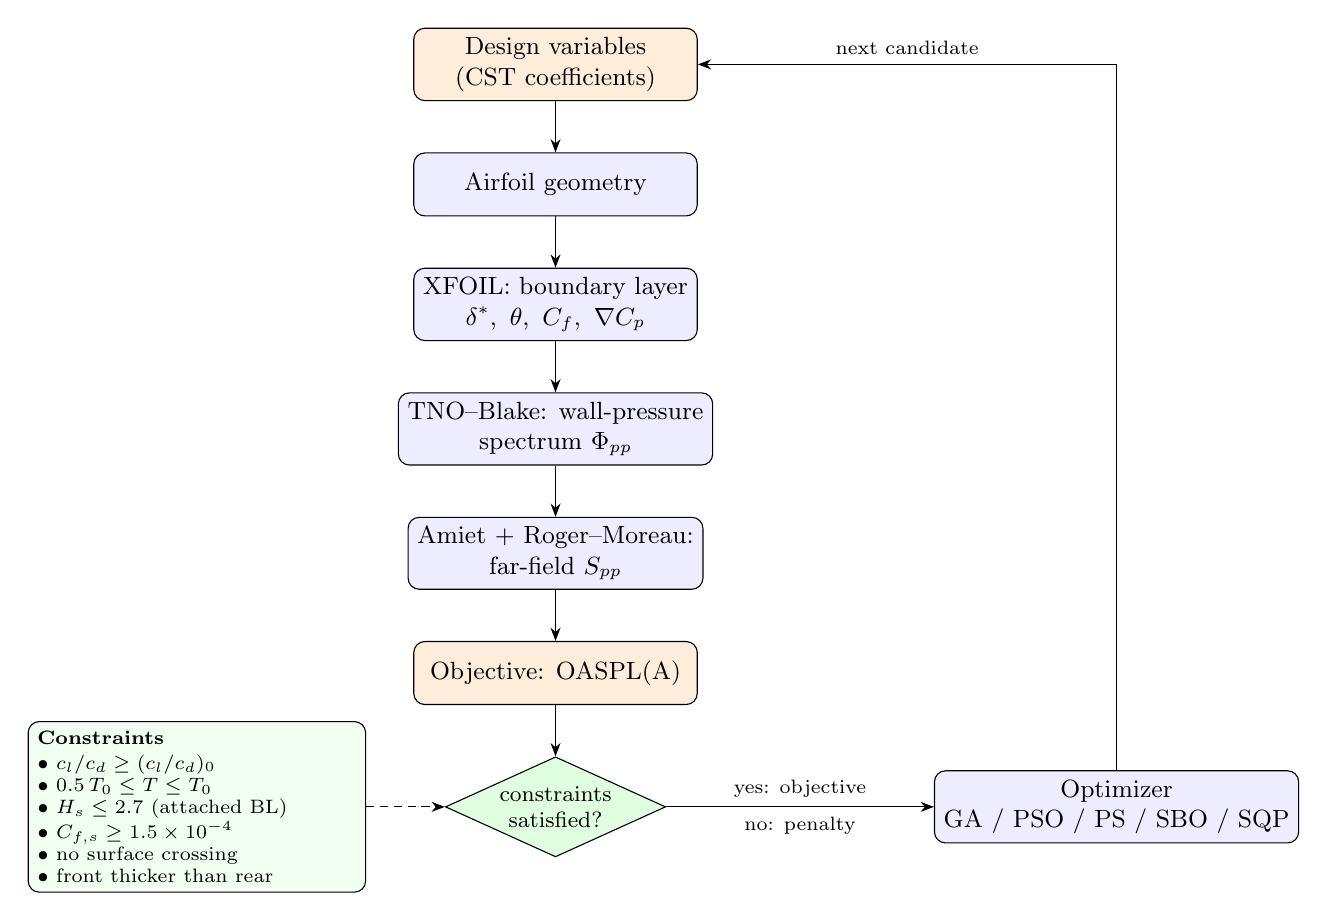
\begin{tikzpicture}[node distance=6.5mm and 16mm, >=Stealth,
  box/.style={draw, rounded corners, align=center, minimum width=3.6cm,
              minimum height=8mm, font=\small},
  proc/.style={box, fill=blue!7},
  io/.style={box, fill=orange!14},
  dec/.style={draw, diamond, aspect=2.2, align=center, fill=green!12,
              font=\footnotesize, inner sep=1pt}]
\node[io]   (dv)    {Design variables\\(CST coefficients)};
\node[proc, below=of dv]    (geo)   {Airfoil geometry};
\node[proc, below=of geo]   (xfoil) {XFOIL: boundary layer\\$\delta^\ast,\ \theta,\ C_f,\ \nabla C_p$};
\node[proc, below=of xfoil] (tno)   {TNO--Blake: wall-pressure\\spectrum $\Phi_{pp}$};
\node[proc, below=of tno]   (amiet) {Amiet + Roger--Moreau:\\far-field $S_{pp}$};
\node[io,   below=of amiet] (oaspl) {Objective: OASPL(A)};
\node[dec,  below=of oaspl] (con)   {constraints\\satisfied?};
\node[proc, right=34mm of con] (opt) {Optimizer\\GA / PSO / PS / SBO / SQP};
\node[box, fill=green!6, align=left, font=\scriptsize, text width=4.05cm,
      left=10mm of con] (cons)
  {\textbf{Constraints}\\[1pt]
   $\bullet$\ $c_l/c_d \ge (c_l/c_d)_0$\\
   $\bullet$\ $0.5\,T_0 \le T \le T_0$\\
   $\bullet$\ $H_s \le 2.7$ (attached BL)\\
   $\bullet$\ $C_{f,s} \ge 1.5\times10^{-4}$\\
   $\bullet$\ no surface crossing\\
   $\bullet$\ front thicker than rear};
\draw[densely dashed,->] (cons) -- (con);
\draw[->] (dv)--(geo); \draw[->] (geo)--(xfoil); \draw[->] (xfoil)--(tno);
\draw[->] (tno)--(amiet); \draw[->] (amiet)--(oaspl); \draw[->] (oaspl)--(con);
\draw[->] (con) -- (opt)
  node[midway,above,font=\scriptsize]{yes: objective}
  node[midway,below,font=\scriptsize]{no: penalty};
% feedback routed up the right side and across the top (avoids the diamond)
\draw[->] (opt.north) |- (dv.east)
  node[near end,above,font=\scriptsize]{next candidate};
\end{tikzpicture}
\caption{Aeroacoustic shape-optimization framework. Each candidate is evaluated
through XFOIL and the Amiet+TNO chain; feasible designs return their OASPL(A) as
the objective value, while infeasible designs (constraint violation or XFOIL
non-convergence) are penalized. The geometric and boundary-layer attachment
constraints enforced at the feasibility check are listed at that node
[cf.\ Eq.~\eqref{eq:problem}]. The optimizer then proposes the next candidate. The
aerodynamic/acoustic models are fixed; the geometry parameterization and the
optimizer are the design choices compared in this work.}
\label{fig:framework}
\end{figure}

\subsection{Geometry parameterization}
Three classical parameterizations were assessed by reconstructing the baseline
airfoil. The Class/Shape Transformation (CST) \citep{Kulfan2006} writes each
surface as
\begin{equation}
\frac{y}{c}=C\!\left(\tfrac{x}{c}\right)S\!\left(\tfrac{x}{c}\right)
+\tfrac{x}{c}\,\tfrac{\Delta z_{te}}{c},\quad
C=\left(\tfrac{x}{c}\right)^{N_1}\!\left(1-\tfrac{x}{c}\right)^{N_2},
\label{eq:cst}
\end{equation}
with $N_1=0.5$, $N_2=1.0$ and $S$ a Bernstein polynomial of order $n$ whose
coefficients are the design variables. PARSEC \citep{Sobieczky1999} builds each
surface from a set of geometric features (leading-edge radius, crest
location/curvature, trailing-edge properties), and Hicks--Henne
\citep{HicksHenne1978} adds bump functions to a baseline surface.
Figure~\ref{fig:paramvars} illustrates, on the baseline section, where the
design variables of each parameterization act: the chordwise stations of the
CST Bernstein coefficients, the geometric features of PARSEC (leading-edge
radius, upper/lower crests and trailing-edge properties), and the bump
locations of Hicks--Henne.

\begin{figure}[!htbp]\centering
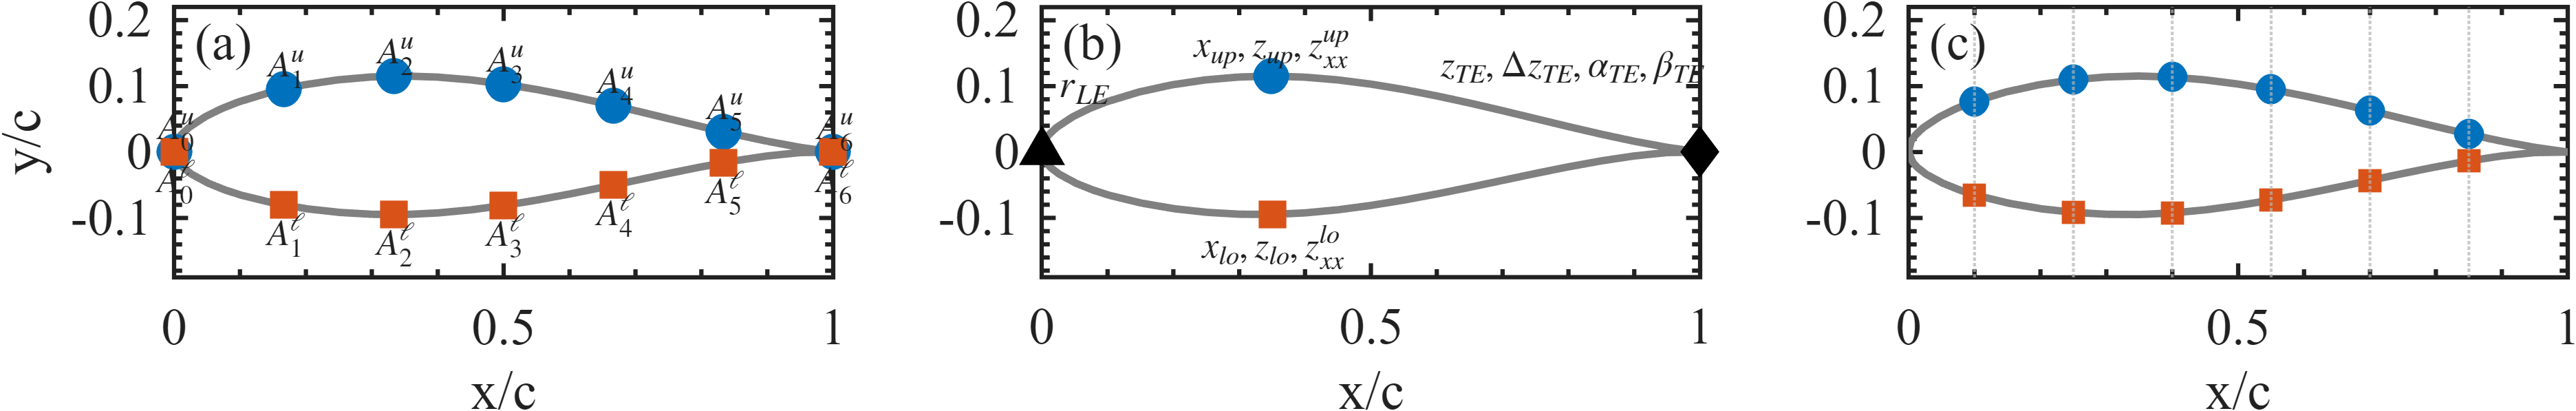
\includegraphics[width=\linewidth]{fig_param_variables.png}
\caption{Design variables of each parameterization on the baseline NACA 63-221
(blue: upper surface, orange: lower surface). (a)~CST: the 14 Bernstein
coefficients ($A^{u}_{0\text{--}6}$, $A^{\ell}_{0\text{--}6}$) at their
chordwise influence stations $x/c=i/6$. (b)~PARSEC geometric features:
leading-edge radius $r_{LE}$, upper/lower crest position, height and curvature
($x,z,z_{xx}$), and trailing-edge thickness/offset/angles
($z_{TE},\Delta z_{TE},\alpha_{TE},\beta_{TE}$). (c)~Hicks--Henne: the
chordwise locations of the bump functions added to the baseline.}
\label{fig:paramvars}
\end{figure}

The three parameterizations are fitted to the baseline NACA 63-221 and compared
by the root-mean-square and maximum chord-normalized surface error,
\begin{equation}
\mathrm{RMSE}=\sqrt{\tfrac{1}{N}\textstyle\sum_i (y_i^{\mathrm{fit}}-y_i^{\mathrm{base}})^2},
\qquad
e_{\max}=\max_i |y_i^{\mathrm{fit}}-y_i^{\mathrm{base}}|,
\end{equation}
evaluated over the union of the cosine-spaced points of both surfaces (equal
weight per point, so the leading- and trailing-edge regions are sampled more
densely). Table~\ref{tab:param} lists the results and
Fig.~\ref{fig:param} shows the reconstructions. CST achieves the lowest error
($\mathrm{RMSE}=2.2\times10^{-4}$) with a compact set of variables; the
least-squares PARSEC basis comes close, while the classical feature-based
PARSEC and Hicks--Henne are roughly five-to-eight times less accurate. This
is a reconstruction-based \emph{screening}, not a comparison of optimization
performance: the parameterizations differ slightly in their number of design
variables (11--14), and a parameterization with a larger reconstruction error
could in principle still span an acoustically favorable design space ---
optimizing with each parameterization under a matched budget is left as
future work. On the screening evidence, CST
is adopted for the optimization (Bernstein order~6, i.e.\ 14 design
variables).

\begin{table}[!htbp]\centering
\caption{Reconstruction error of the baseline NACA 63-221 (chord-normalized).}
\label{tab:param}
\begin{tabular}{@{}lccc@{}}
\toprule
Method & Design variables & RMSE & $e_{\max}$ \\
\midrule
CST (order 6)            & 14 & $2.2\times10^{-4}$ & $8.5\times10^{-4}$ \\
PARSEC (geometric)       & 11 & $1.7\times10^{-3}$ & $4.8\times10^{-3}$ \\
PARSEC (least-squares)   & 12 & $3.2\times10^{-4}$ & $1.1\times10^{-3}$ \\
Hicks--Henne             & 12 & $1.0\times10^{-3}$ & $5.4\times10^{-3}$ \\
\bottomrule
\end{tabular}
\end{table}

\begin{figure}[!htbp]\centering
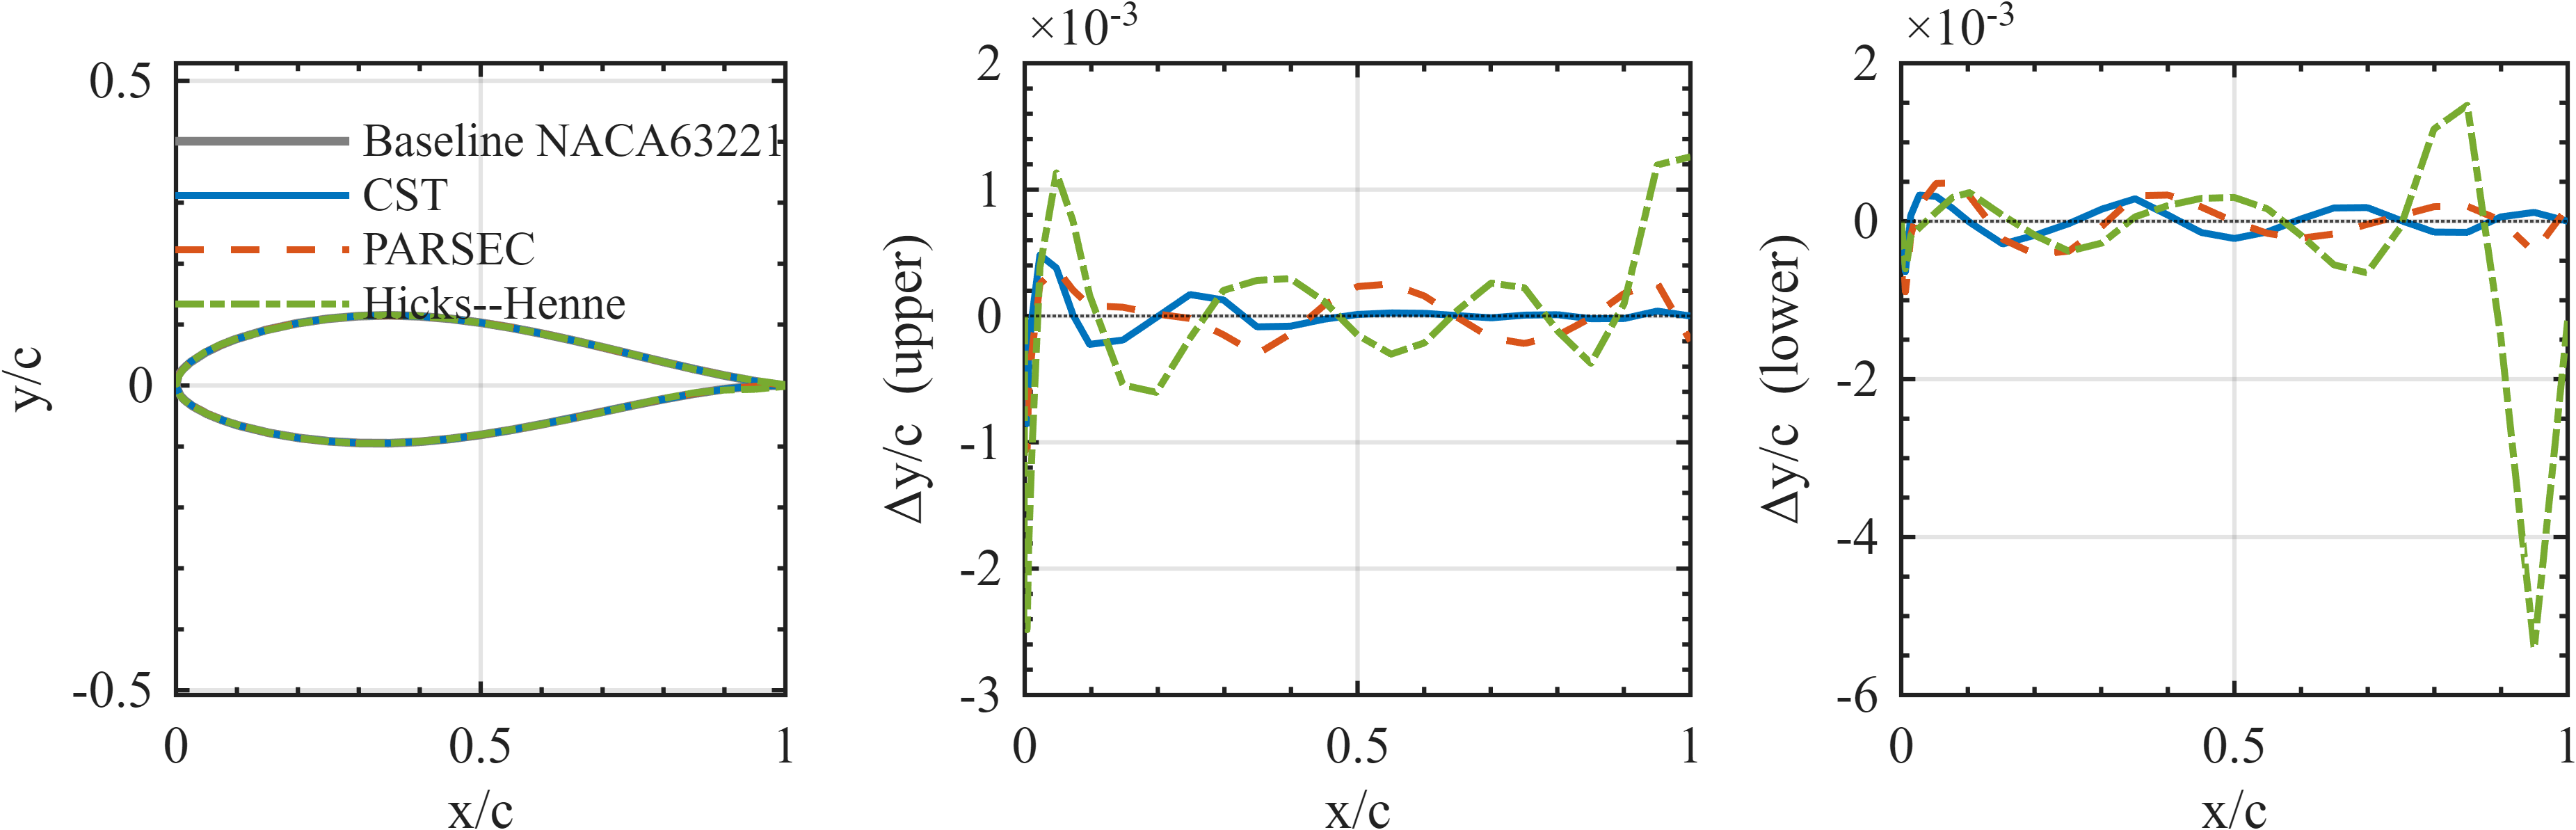
\includegraphics[width=\linewidth]{parameterization_comparison.png}
\caption{Reconstruction of the baseline NACA 63-221 by CST, PARSEC and
Hicks--Henne: (left) geometry overlay, (center) upper-surface error, (right)
lower-surface error.}
\label{fig:param}
\end{figure}

\subsection{Sensitivity analysis}
A one-at-a-time sweep of each CST coefficient across its optimization bound
quantifies its influence on the OASPL(A) (Fig.~\ref{fig:sens}). The largest
variation of the objective occurs when perturbing the high-order (rear)
coefficients of both surfaces --- most strongly the aft suction side, but also
the aft pressure side --- i.e.\ the trailing-edge region where the boundary
layer develops, while the forward coefficients are nearly inactive. The
locally responsive portion of the tested design space is thus concentrated in
a subset of (mostly aft) coefficients, which is exploited to
bound the search. It should be noted that this ranking identifies the most
\emph{influential} geometric degrees of freedom; which surface actually carries
the noise reduction is surface-dependent and is interpreted in
Section~\ref{sec:res} through the wall-pressure spectra.

\begin{figure}[!htbp]\centering
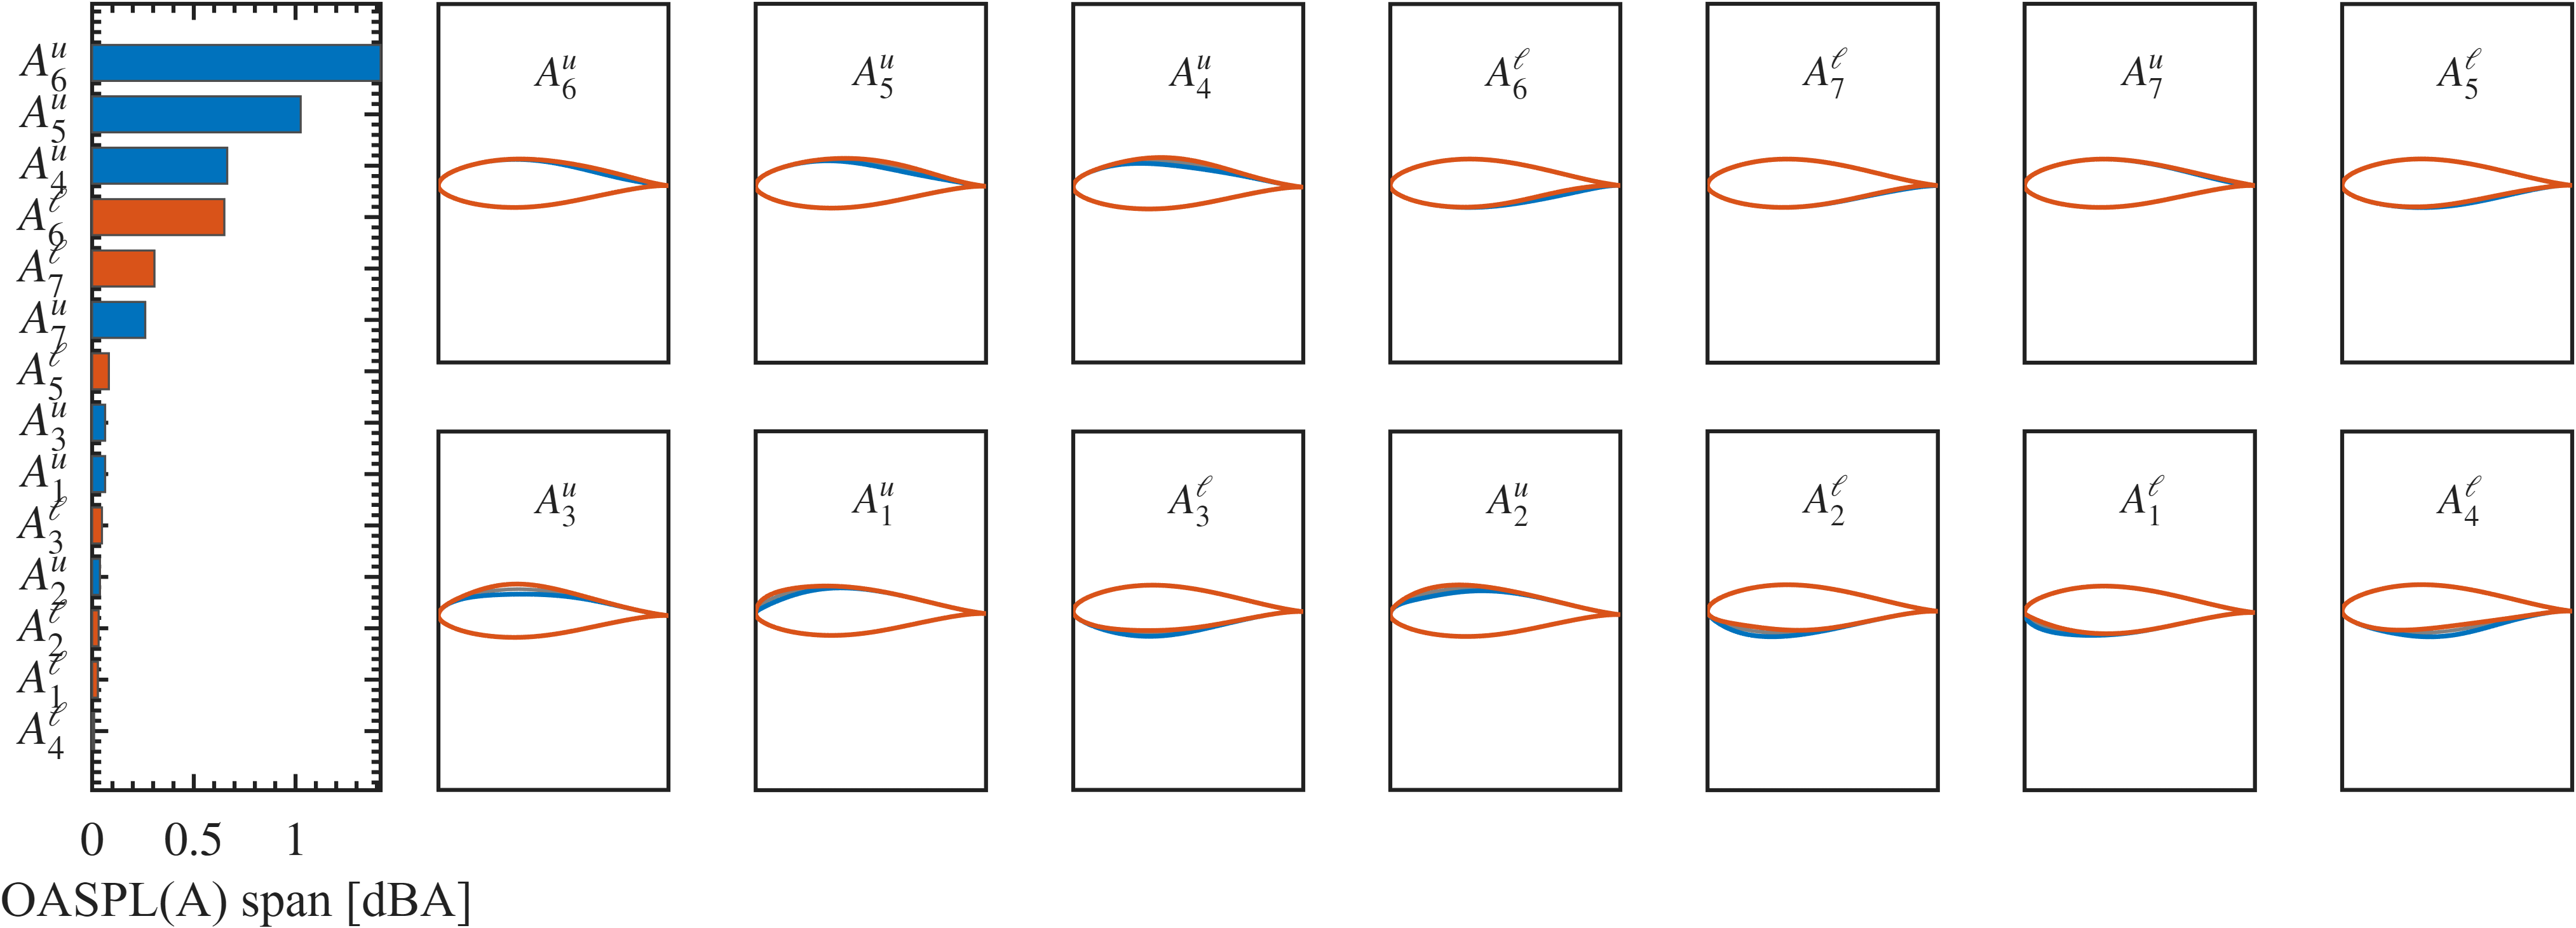
\includegraphics[width=\linewidth]{fig_sensitivity_modes.png}
\caption{Sensitivity of the OASPL(A) to the CST design variables.
(a)~One-at-a-time influence: the bar is the span
$\max(\mathrm{OASPL})-\min(\mathrm{OASPL})$ obtained by sweeping one coefficient
within its $\pm50\%$ bound while holding the others fixed (blue: upper surface,
orange: lower surface); only geometrically feasible, XFOIL-converged candidates
satisfying the attachment constraint are included. (b)~Geometry deformation of
each of the 14 CST modes, ordered by influence (grey: baseline; blue: $-$,
orange: $+$ perturbation). The larger span of the aft coefficients reflects
their stronger, but still physical, effect on the trailing-edge boundary layer.}
\label{fig:sens}
\end{figure}

Being one-at-a-time, this analysis does not capture interactions between
coefficients and the feasible fraction of each sweep differs between
variables; it is therefore used as a preliminary indication of where the
objective is most responsive, not as a formal (e.g.\ Morris- or Sobol-type)
global sensitivity analysis.

\subsection{Optimization algorithms}
Because the objective is non-smooth and expensive (each evaluation runs XFOIL),
derivative-free global methods are preferred. We benchmark five algorithms
widely used in aerodynamic shape optimization: the genetic algorithm (GA)
\citep{Holland1992}, particle swarm optimization (PSO)
\citep{Kennedy1995}, generalized pattern search (PS) \citep{AudetDennis2002},
surrogate-based optimization (SBO) designed for expensive functions
\citep{Jones1998}, and sequential quadratic programming (SQP) as a
gradient-based baseline. All algorithms start from the same point (the CST fit
of the baseline), use the same box bounds ($\pm50\%$ of the baseline
coefficients) and the same evaluation budget, and handle constraints by a
penalty method: candidates that violate the geometric or attachment constraints
or for which XFOIL fails to converge are assigned a large penalty objective, so
the formulation is identical for all solvers, including those without native
constraint support. Their main settings are listed in
Table~\ref{tab:optparams}; the implementation uses the MATLAB Global
Optimization Toolbox (surrogate optimization uses a radial-basis-function
surrogate \citep{Gutmann2001}).

\begin{table}[!htbp]\centering
\caption{Main settings of the optimization algorithms (MATLAB Global
Optimization / Optimization Toolbox). Nominal target budget = 150 objective
evaluations (actual model calls 132--180, see Table~\ref{tab:algo}). Solver
options not listed were left at their R2025b defaults.}
\label{tab:optparams}
\begin{tabular}{@{}lll@{}}
\toprule
Algorithm & Key parameters & Constraints \\
\midrule
Genetic algorithm (GA)   & population 30, seeded with baseline       & penalty \\
Particle swarm (PSO)     & swarm 30, seeded with baseline            & penalty \\
Pattern search (PS)      & complete poll, mesh tol.\ $10^{-4}$       & penalty / nonlinear \\
Surrogate optim.\ (SBO)  & RBF surrogate, baseline as initial point  & penalty \\
SQP (fmincon)            & finite-difference gradients               & penalty \\
\bottomrule
\end{tabular}
\end{table}

\subsection{Problem formulation}
Following \citet{Kou2023}, the noise objective is minimized subject to
aerodynamic and geometric constraints,
\begin{equation}
\begin{aligned}
\min_{\mathbf{a}}\ & \mathrm{OASPL(A)}(\mathbf{a}),\quad\text{s.t.}\quad
\frac{c_l}{c_d}\ge\left(\frac{c_l}{c_d}\right)_{\!0},\quad
0.5\,T_0\le T\le T_0+\varepsilon_T,\\[2pt]
& \min_x(y_u-y_l)\ge\varepsilon_g,\quad
T_\mathrm{LE}\ge T_\mathrm{TE},\quad
H_s\le H_{\!\lim},\quad
C_{f,s}\ge C_{f,\min},
\end{aligned}
\label{eq:problem}
\end{equation}
where $\mathbf{a}$ are the CST coefficients, the subscript $0$ denotes the
baseline, $T$ is the maximum thickness, and $T_\mathrm{LE}$, $T_\mathrm{TE}$ are
the maximum thicknesses of the front and rear halves (separated at $x/c=0.5$;
this condition excludes aft-loaded thickness distributions as a design
preference for blade-like sections --- no structural analysis is implied).
The
minimum-separation and cap tolerances are $\varepsilon_g$ and $\varepsilon_T$;
in the present implementation the local thickness is tested on the
cosine-spaced CST grid with $\varepsilon_g=-10^{-4}c$ (a small tolerance that
admits at most $10^{-4}c$ of local overlap on that grid, avoiding spurious
rejection of otherwise valid shapes) and $\varepsilon_T=10^{-3}c$; the
minimum-thickness floor $0.5\,T_0$ is a geometric bound, not a demonstrated
structural requirement. Both reported optima have strictly positive local
thickness everywhere, so no surface crossing occurs at the solutions; a
strictly positive $\varepsilon_g$ evaluated on a denser geometric grid would
be a cleaner enforcement and is noted as a refinement. The last two conditions of Eq.~\eqref{eq:problem}
are an \emph{attachment constraint}: $H_s$ and $C_{f,s}$ are the suction-side
shape factor and skin-friction coefficient at the wall-pressure sampling station
($x/c=0.99$), bounded by $H_{\!\lim}=2.7$ and $C_{f,\min}=1.5\times10^{-4}$.
The shape-factor bound sits in the commonly quoted range $H\approx2.5$--$3$
for incipient turbulent separation, and the skin-friction floor lies just
below the baseline value while remaining well above zero; both are checked at
the station that feeds the acoustic model.
Because the TNO model assumes an attached turbulent boundary layer, without this
constraint the optimizer lowers the predicted wall pressure by driving the
suction side toward separation ($H\!\to\!$ large, $C_f\!\to\!0$), exploiting the
model outside its range of validity; the attachment constraint keeps every
accepted candidate within that range. The CST coefficients are allowed to vary
within $\pm 50\%$ of the baseline values (with an absolute half-width floor of
$0.05$ for near-zero coefficients) --- a wider box than the $\pm30\%$ of \citet{Kou2023};
Section~\ref{sec:res} quantifies how the attainable reduction grows with the
box width, and the $\pm50\%$ box is adopted as a compromise between design
freedom and geometric proximity to the baseline family; the geometric constraints
(no surface crossing, thickness cap and front-heavier-than-rear) keep every
candidate geometrically admissible within the present two-dimensional
optimization framework. Two variants are solved: a single-objective problem with
the efficiency constraint enforced as a hard constraint, and a multi-objective
problem yielding the noise--efficiency Pareto front.

The single-objective optimizer (pattern search) stops at the first of two
criteria: a mesh tolerance of $10^{-4}$ (the search refines a mesh whose size
decreases as it approaches a local optimum) or a maximum number of XFOIL
evaluations. For the algorithm comparison, a nominal evaluation budget is used
as the common stopping criterion (the number of calls actually issued varies
with the algorithm class; Section~\ref{sec:algos}), and the
multi-objective optimizer (MATLAB \texttt{gamultiobj}, an NSGA-II-type
algorithm; population 40, 30 generations, intermediate crossover, remaining
settings at their R2025b defaults) is run for a fixed number of generations. The
operating and numerical conditions of the optimization case are summarized in
Table~\ref{tab:cond}, and the parameters of each optimizer in
Table~\ref{tab:optparams}. The inflow velocity of \SI{83.31}{m/s} represents the
relative velocity at an outboard wind-turbine blade section (not the free-stream
wind speed), and the angle of attack of \ang{4} is the design incidence of the
NACA 63-221 at this Reynolds number: it gives a high lift-to-drag ratio while
keeping the suction-side boundary layer attached (higher incidences separate
near the trailing edge for this thick section).

\begin{table}[!htbp]\centering
\caption{Operating and numerical conditions of the optimization case.}
\label{tab:cond}
\begin{tabular}{@{}llll@{}}
\toprule
Parameter & Value & Parameter & Value \\
\midrule
Baseline airfoil       & NACA 63-221        & Air density $\rho$    & \SI{1.181}{kg/m^3} \\
Chord $c$              & \SI{0.57}{m}       & Speed of sound $c_0$  & \SI{344}{m/s} \\
Span $b$               & \SI{1}{m}          & Kinematic visc.\ $\nu$& \SI{1.5e-5}{m^2/s} \\
Inflow $U_\infty$      & \SI{83.31}{m/s}    & Temperature           & \SI{22}{\celsius} \\
Angle of attack        & \ang{4}            & Wall-pressure model   & TNO--Blake \\
Reynolds $Re$          & $3.17\times10^6$   & Wall-pressure $x/c$   & 0.99 \\
Mach $M$               & 0.24               & CST surface points    & 100 (cosine) \\
Transition $x/c$ (both)& 0.05               & XFOIL iterations      & 1000 \\
Observer $(x,y,z)$     & $(0,0,1)$~m        & Frequency range       & \SIrange{100}{20000}{Hz} \\
\bottomrule
\end{tabular}
\end{table}

%========================================================================
\section{Results and discussion}\label{sec:res}
%========================================================================
\subsection{Optimized geometry and spectrum}
The single-objective optimization, carried out with pattern search (used as the
dedicated single-objective optimizer for its robustness on the non-smooth
objective and run to a larger evaluation budget than the algorithm benchmark of
Section~\ref{sec:algos}), reduces the OASPL(A) of the baseline NACA 63-221 from
\SI{67.10}{dBA} to \SI{65.82}{dBA}, a reduction of \SI{1.28}{dBA} (about
\SI{26}{\percent} of the A-weighted mean-square acoustic pressure), while slightly improving
the lift-to-drag ratio ($c_l/c_d$ from $54.2$ to $54.8$), above the constraint
floor. The optimized design therefore dominates the baseline: it is quieter
without a lift-to-drag penalty at the prescribed operating point. The run
terminated on the mesh-tolerance criterion rather than on the evaluation budget
(which, for a non-smooth XFOIL-in-the-loop objective with penalty terms,
indicates a converged search rather than a certified local minimizer).

Figure~\ref{fig:mechgeom} shows the geometric change. In contrast to what is
often reported for thinner sections, the optimizer does \emph{not} thin the
airfoil: the maximum thickness stays close to its cap ($t_{\max}/c$ from
$0.210$ to $0.205$, panel c, within \SI{2.4}{\percent} of the bound).
Instead, it reshapes the section at approximately constant thickness --- the maximum
camber quadruples (from $0.011$ to $0.046$, panel d) and moves forward (from
$x/c\approx0.54$ to $0.30$), producing a more front-loaded section. The added
camber raises the lift ($c_l$ from $0.630$ to $0.713$) at a modest drag penalty
($c_d$ from $0.0116$ to $0.0130$), leaving the lift-to-drag ratio slightly
improved, and the pitching-moment magnitude decreases ($c_m$ from $-0.038$ to
$-0.013$). Because the maximum thickness remains within \SI{2.4}{\percent} of
the baseline value, the sectional depth available for structure is
essentially retained --- a practically relevant property for a midboard
blade station (the thickness \emph{distribution} does change moderately over
the rear half, Fig.~\ref{fig:mechgeom}c). The most modified coefficients are those of the pressure surface
and the aft suction surface (Fig.~\ref{fig:modes}), consistent with the
sensitivity analysis.

Splitting the OASPL by surface clarifies the mechanism. In contrast to thin
sections, for this thick \SI{21}{\percent} airfoil the \emph{pressure} side is
the dominant far-field source: it carries the higher wall-pressure spectral peak
(\SI{76.4}{dB} versus \SI{73.6}{dB} on the suction side, Table~\ref{tab:bl}) and
its isolated contribution (\SI{65.9}{dBA}) is some \SI{5}{dBA} above that of the
suction side (\SI{60.9}{dBA}). The optimization lowers \emph{both} surfaces, by
very different decibel amounts: the suction-side contribution drops from
\SI{60.9}{dBA} to \SI{56.8}{dBA}, while the pressure-side contribution decreases
from \SI{65.9}{dBA} to \SI{65.2}{dBA}. The total is the incoherent
(mean-square) sum of the two contributions,
$\mathrm{OASPL}=10\log_{10}(10^{L_s/10}+10^{L_p/10})$, the standard
assumption in Amiet-type predictions since the turbulent boundary layers on
opposite surfaces are statistically independent
\citep{RogerMoreau2005}. In energy terms the two
changes are
comparable --- the large decibel drop of the quieter suction side carries about
\SI{56}{\percent} of the \SI{1.28}{dBA} overall decrease, and the smaller
decibel change of the dominant pressure side the remaining \SI{44}{\percent}
(fractions computed from the one-decimal levels quoted above).
Crucially, the suction-side boundary layer remains \emph{attached}: the shape
factor rises from $H=2.26$ to $H=2.62$ --- still below the imposed limit
$H_{\!\lim}=2.7$ --- and the skin friction sits at the floor ($C_f$ from
$3.3\times10^{-4}$ to $1.5\times10^{-4}$), the attachment constraint being
active at the optimum. The noise reduction is thus obtained from genuinely lower
wall-pressure spectra on an attached boundary layer (peak level \SI{73.6}{dB} to
\SI{70.3}{dB} on the suction side and \SI{76.4}{dB} to \SI{75.6}{dB} on the
pressure side), not by exploiting the TNO model near separation. During the
optimization the constraint is enforced on the suction side at the sampling
station only; for the reported baseline and optimum the full chordwise
distributions (Fig.~\ref{fig:cfh}) show that, downstream of the trip, the
most restrictive values of $H$ and $C_f$ occur near the trailing edge on both
surfaces, with no upstream separation --- although this behavior was not
formally verified for every evaluated candidate, and extending the constraint
to both surfaces over the whole chord is a natural improvement. This is the key
methodological safeguard discussed in Section~\ref{sec:concl}.

\begin{figure}[!htbp]\centering
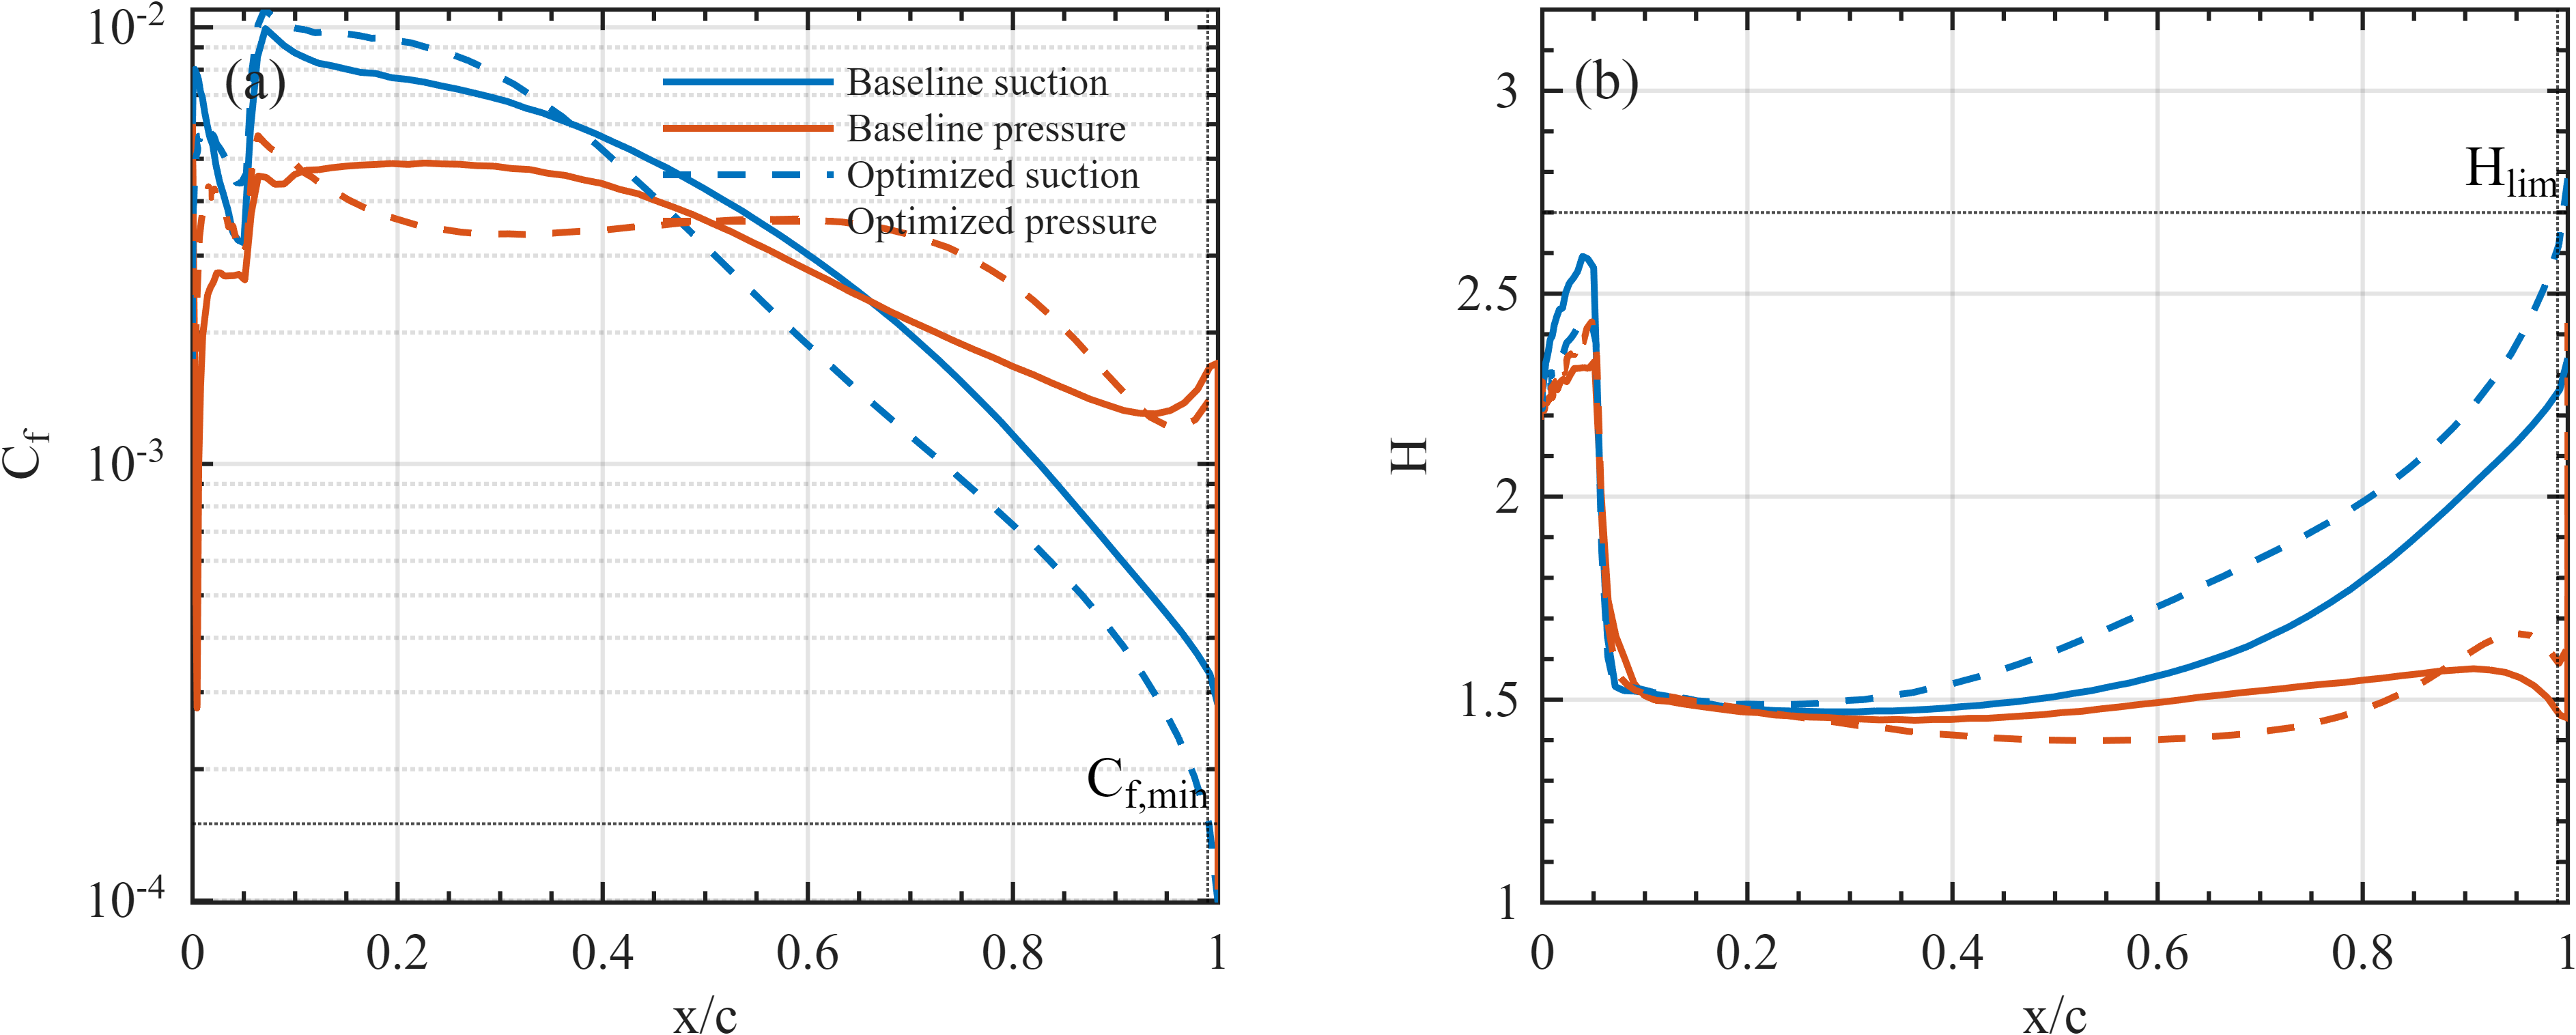
\includegraphics[width=\linewidth]{fig_cfh_NACA63221.png}
\caption{Chordwise skin-friction (a) and shape-factor (b) distributions of the
baseline and optimized NACA 63-221 on both surfaces, with the attachment
bounds $C_{f,\min}$ and $H_{\lim}$ and the sampling station $x/c=0.99$
(dotted). Both surfaces remain attached along the entire chord; the
corresponding distributions of the 63-218 case are analogous.}
\label{fig:cfh}
\end{figure}

\begin{table}[!htbp]\centering
\caption{Boundary-layer parameters at the wall-pressure sampling location
$x/c=0.99$ for the baseline and optimized airfoils ($\delta^\ast$ and $\theta$
normalized by chord; $\Phi_{pp,\mathrm{pk}}$ is the peak wall-pressure spectral
level in $\mathrm{dB\ re}\ (20\,\mu\mathrm{Pa})^2/\mathrm{Hz}$, the reference
used in all spectral figures).}
\label{tab:bl}
\begin{tabular}{@{}llrrrrrr@{}}
\toprule
Case & Surface & $\delta^\ast/c$ & $\theta/c$ & $H$ & $C_f$ & $U_e/U_\infty$ & $\Phi_{pp,\mathrm{pk}}$ [dB] \\
\midrule
baseline  & suction  & 0.0149 & 0.0066 & 2.26 & 0.00033 & 0.869 & 73.6 \\
baseline  & pressure & 0.0042 & 0.0029 & 1.46 & 0.00167 & 0.861 & 76.4 \\
optimized & suction  & 0.0213 & 0.0081 & 2.62 & 0.00015 & 0.861 & 70.3 \\
optimized & pressure & 0.0042 & 0.0026 & 1.59 & 0.00140 & 0.872 & 75.6 \\
\bottomrule
\end{tabular}
\end{table}

Figure~\ref{fig:spec} shows that the far-field noise is reduced across most of
the frequency range --- most strongly at low-to-mid frequencies and only
marginally at high frequency --- not only in the integrated value.

To quantify how the reduction depends on the allowed design freedom, the design
box was progressively widened. With bounds of $\pm30\%$, $\pm50\%$ and
$\pm70\%$ on the CST coefficients, the optimized reduction is \SI{1.02}{dBA},
\SI{1.28}{dBA} and \SI{1.74}{dBA} respectively: wider boxes admit quieter
designs, but through geometries that depart progressively further from the
63-221 family (the $\pm70\%$ optimum abandons the thickness cap and thins the
section to $t_{\max}/c=0.17$). The $\pm50\%$ box is therefore a design choice
that balances noise reduction against geometric fidelity to the baseline
family, and the quoted reduction should be read as conditional on that choice.
The multi-objective
front of Section~\ref{sec:pareto}, which does \emph{not} enforce the
lift-to-drag constraint, reaches essentially the same level
(\SI{65.96}{dBA} against \SI{65.82}{dBA}); this independent search provides a
consistency check that the constrained optimum is not limited by the
aerodynamic constraint, although it does not establish global optimality. The modest
decibel figure is a property of the case --- a thick section at a fixed, fully
turbulent operating point --- and of the chosen design freedom, not of the
optimizer.

\begin{figure}[!htbp]\centering
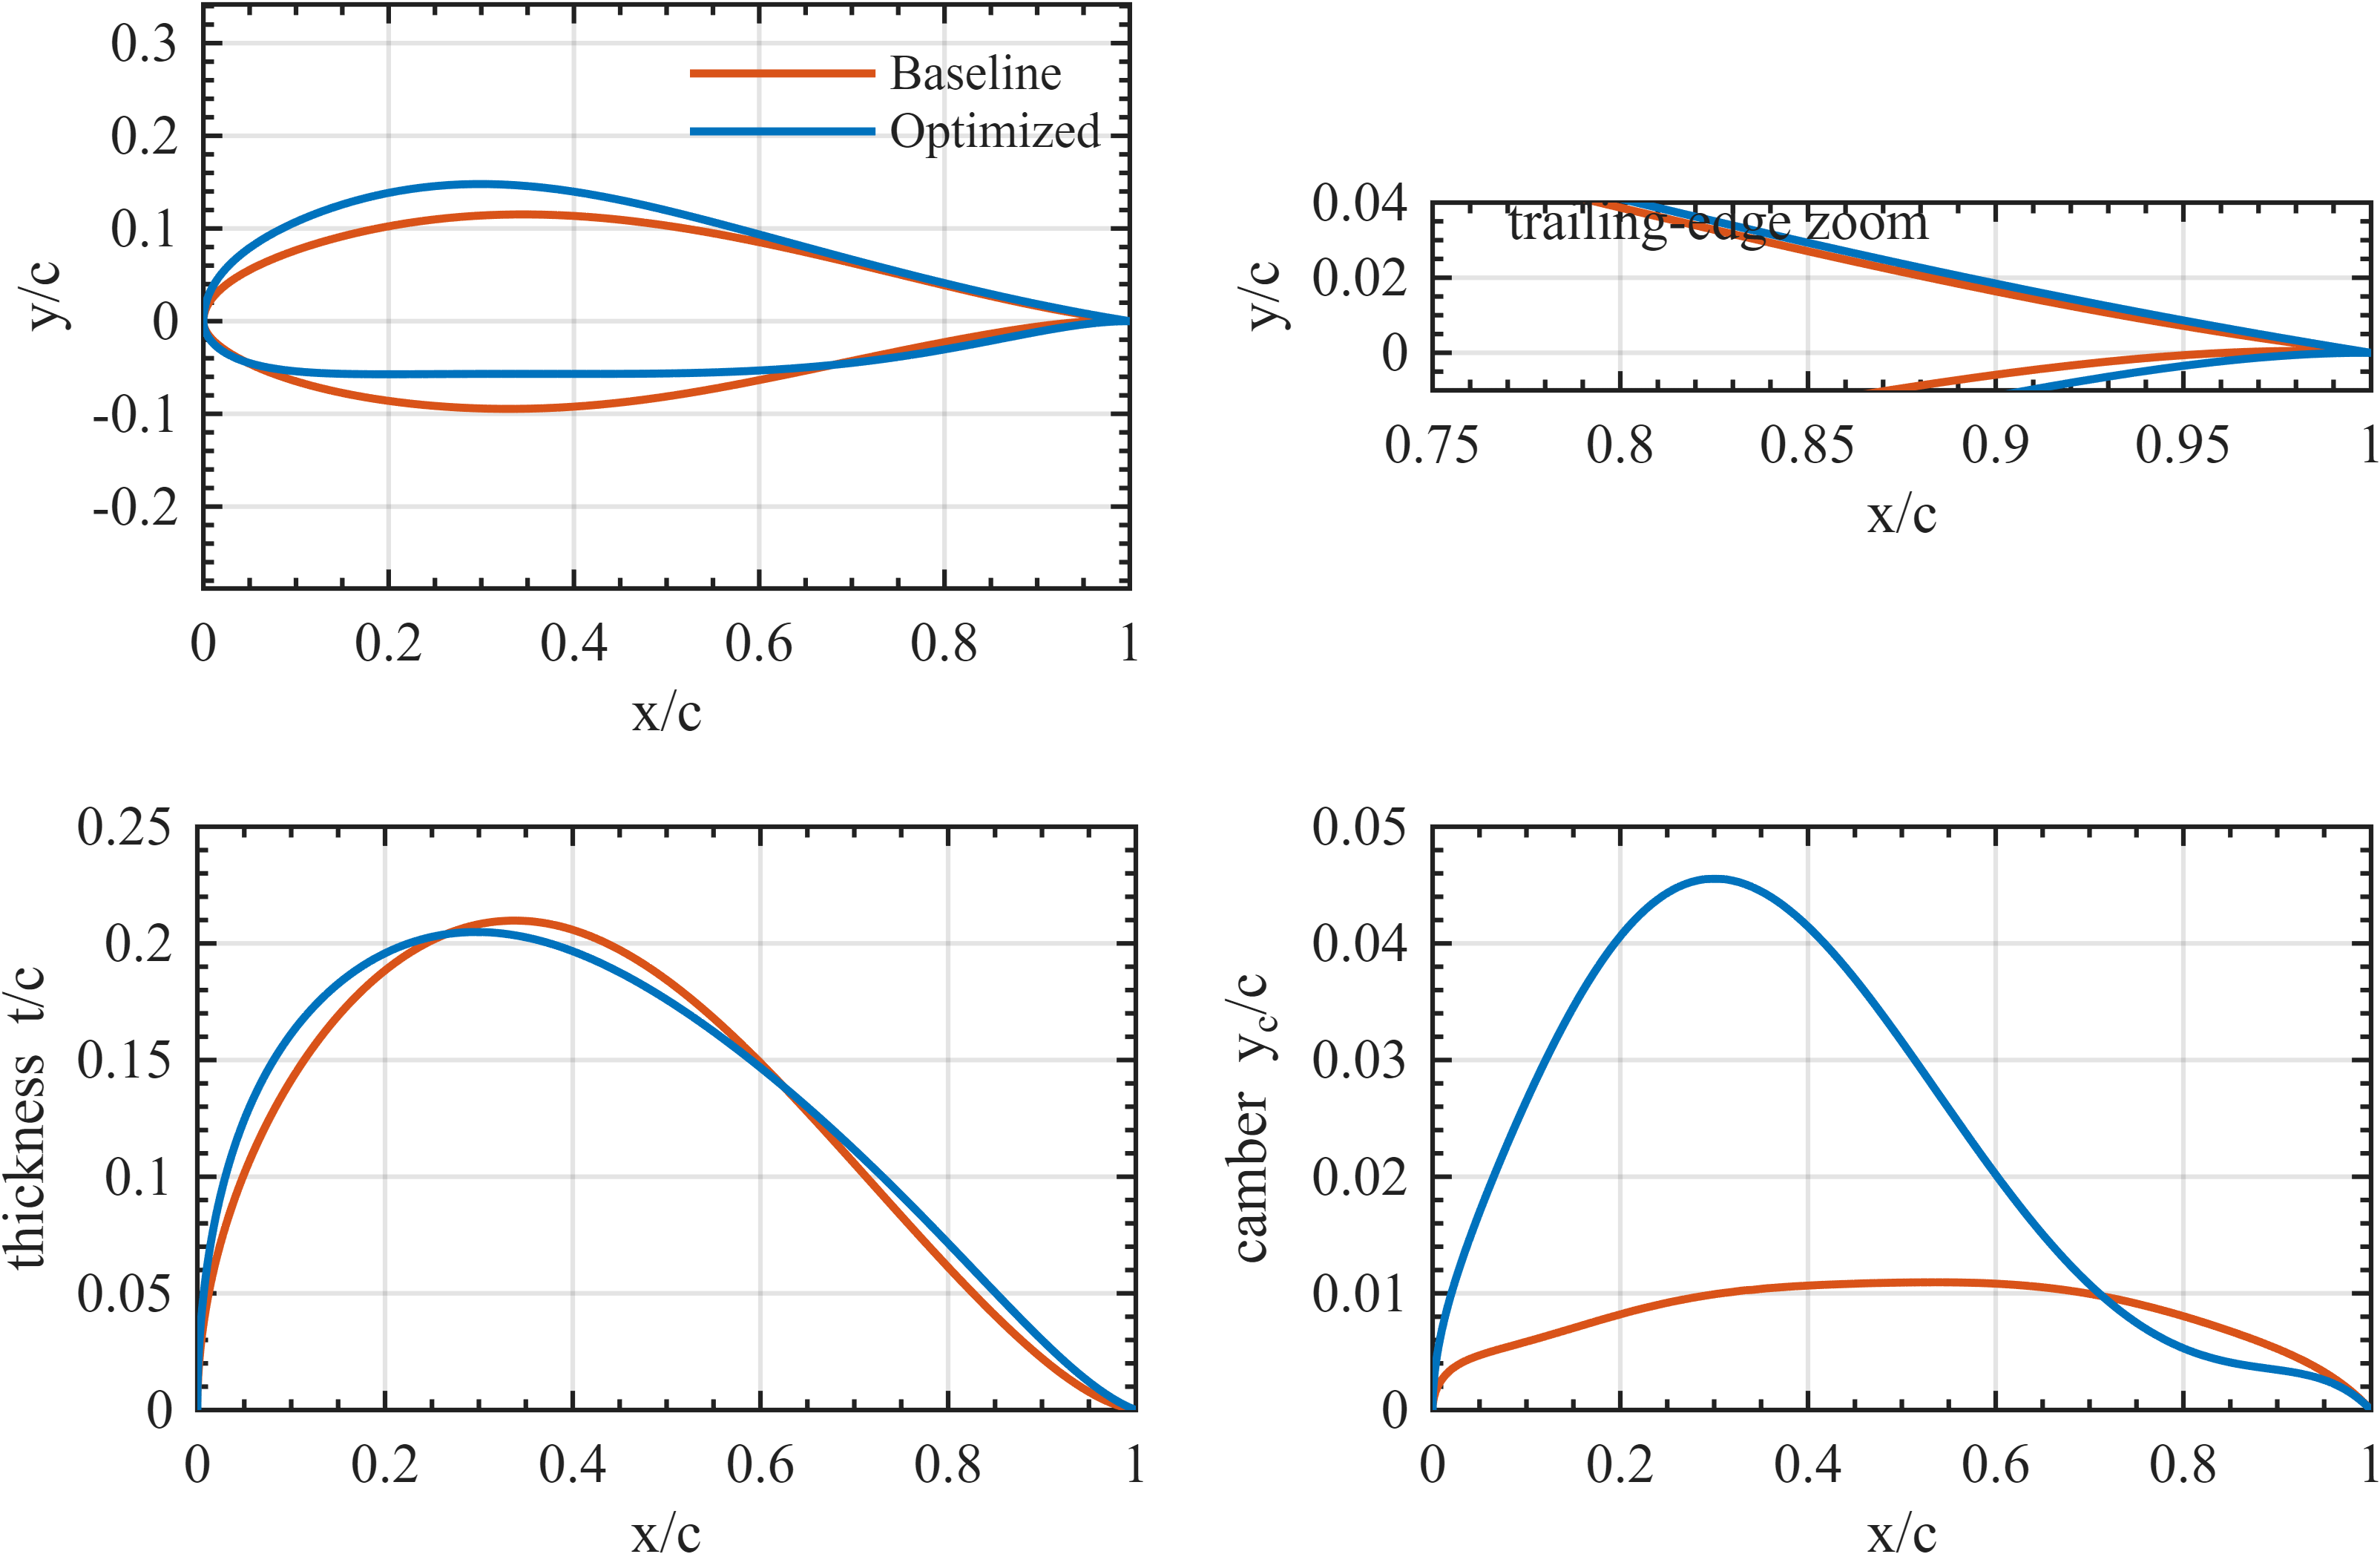
\includegraphics[width=0.85\linewidth]{fig_mechanism_geom.png}
\caption{Geometric change behind the noise reduction (orange: baseline, blue:
optimized): (a) baseline versus optimized silhouette; (b) trailing-edge zoom;
(c) thickness $t/c$; (d) camber line.}
\label{fig:mechgeom}
\end{figure}

\begin{figure}[!htbp]\centering
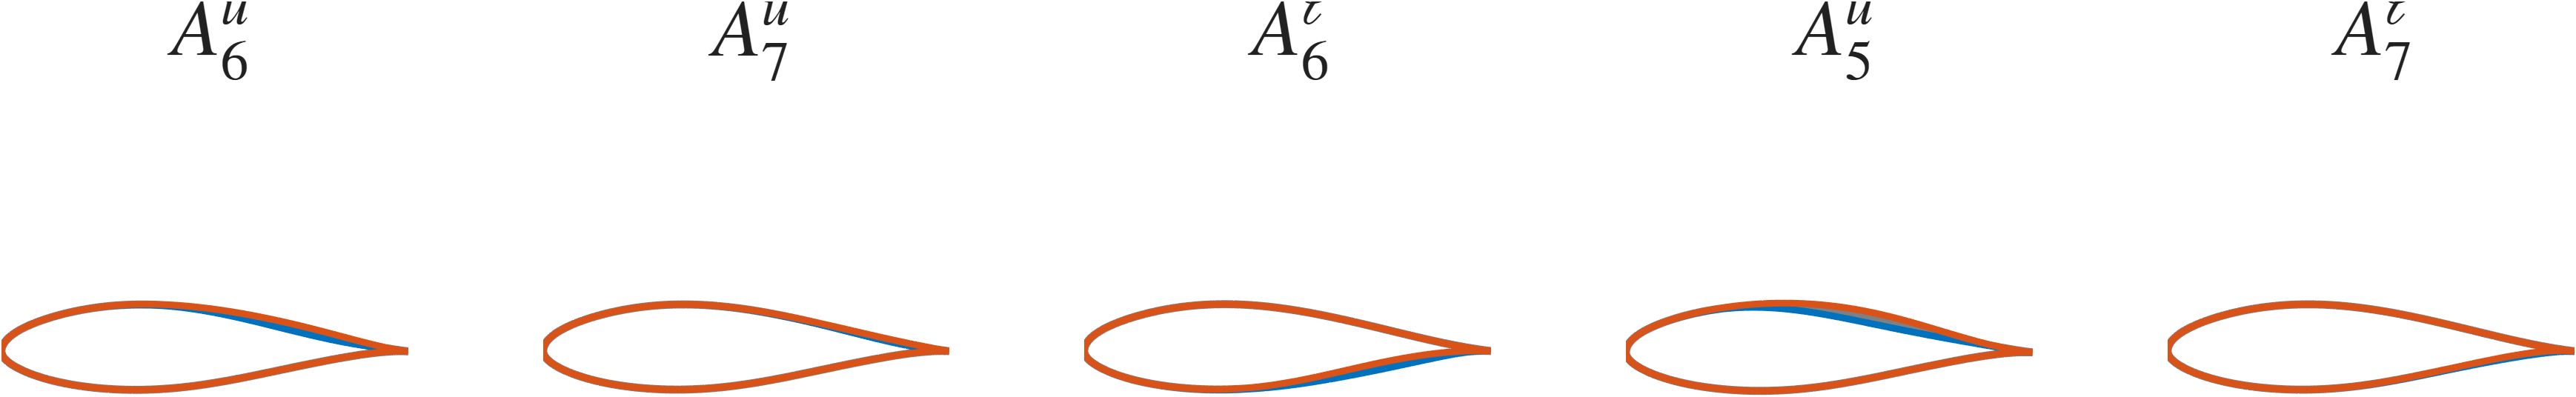
\includegraphics[width=\linewidth]{fig_shape_modes_top.png}
\caption{Geometry deformation produced by the five most influential CST modes
(grey: baseline; blue: $-$, orange: $+$ perturbation). The full set of modes
and their ranked influence are given in Fig.~\ref{fig:sens}(b).}
\label{fig:modes}
\end{figure}

\begin{figure}[!htbp]\centering
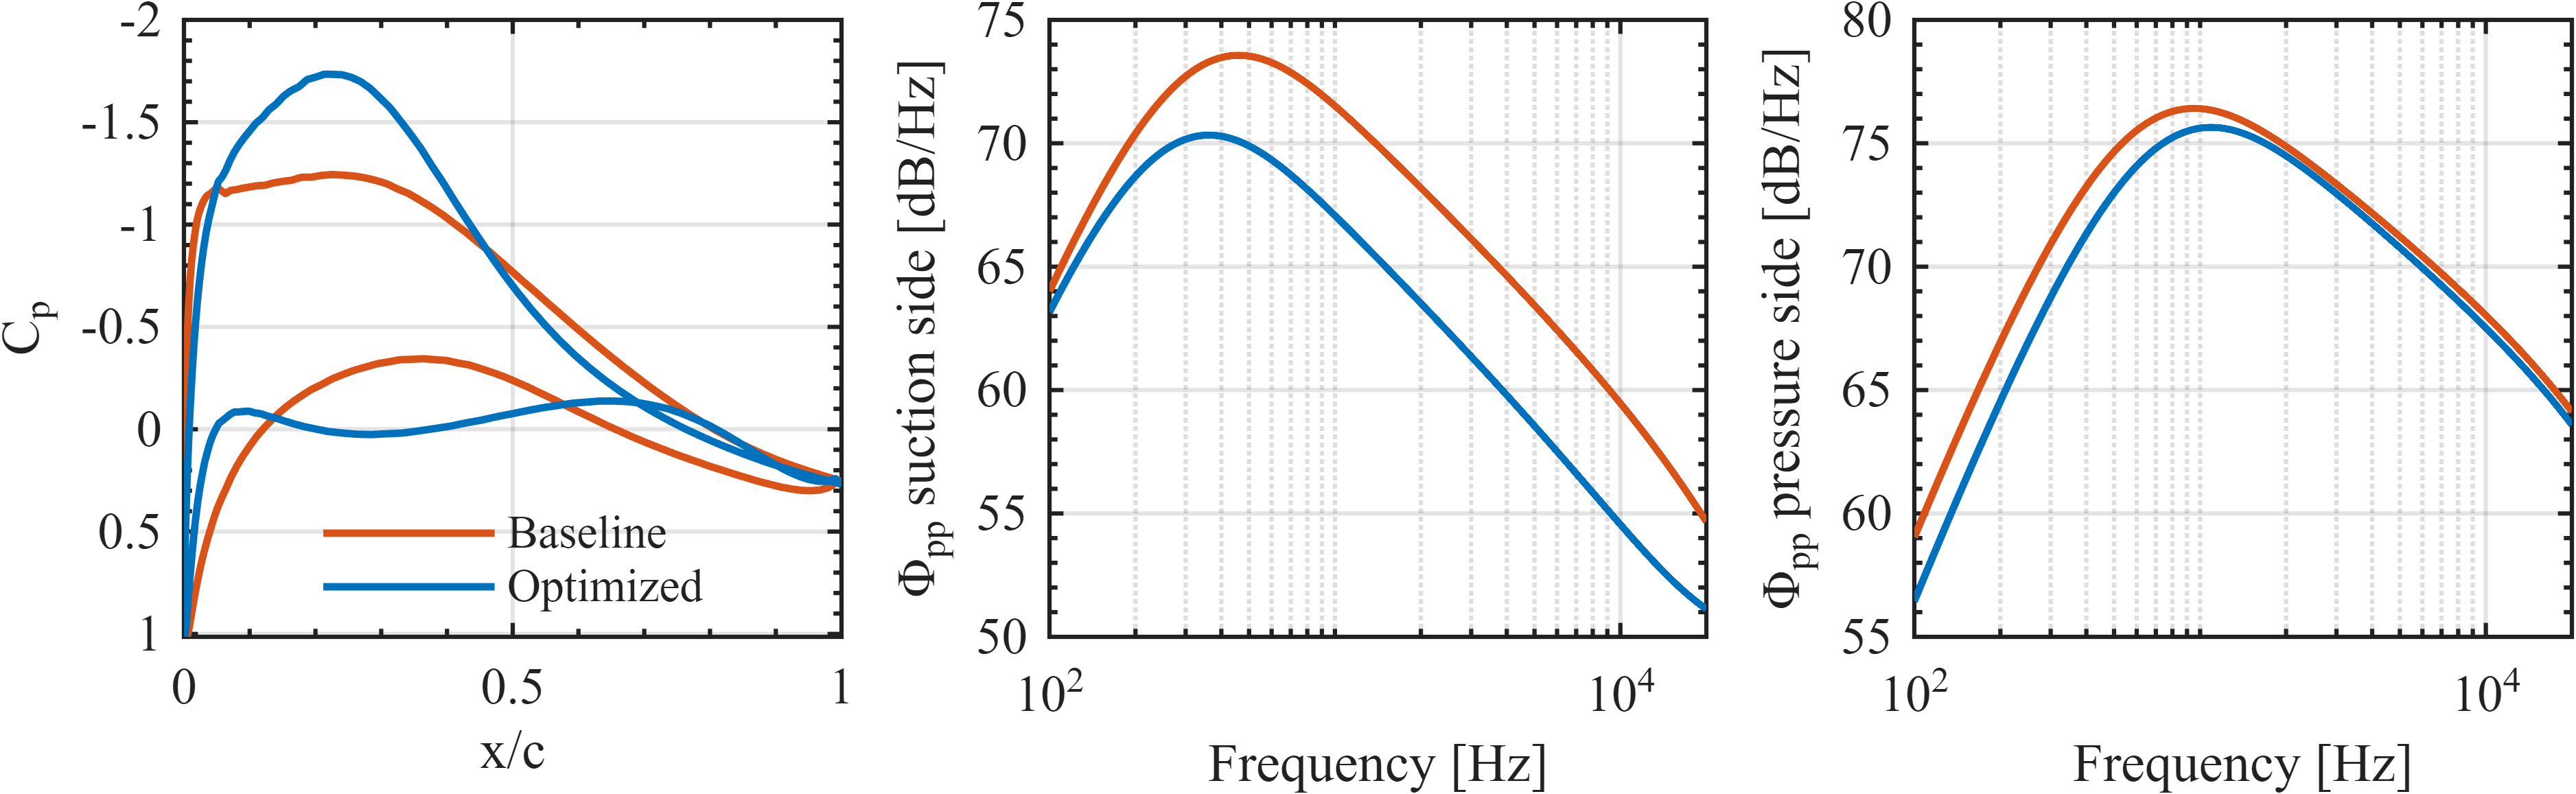
\includegraphics[width=\linewidth]{fig_mechanism_aero.png}
\caption{Aerodynamic and acoustic mechanism (baseline versus optimized): (left)
surface pressure coefficient $C_p$; (center) suction-side and (right)
pressure-side wall-pressure spectrum at $x/c=0.99$, the far-field source term.}
\label{fig:mechaero}
\end{figure}

\begin{figure}[!htbp]\centering
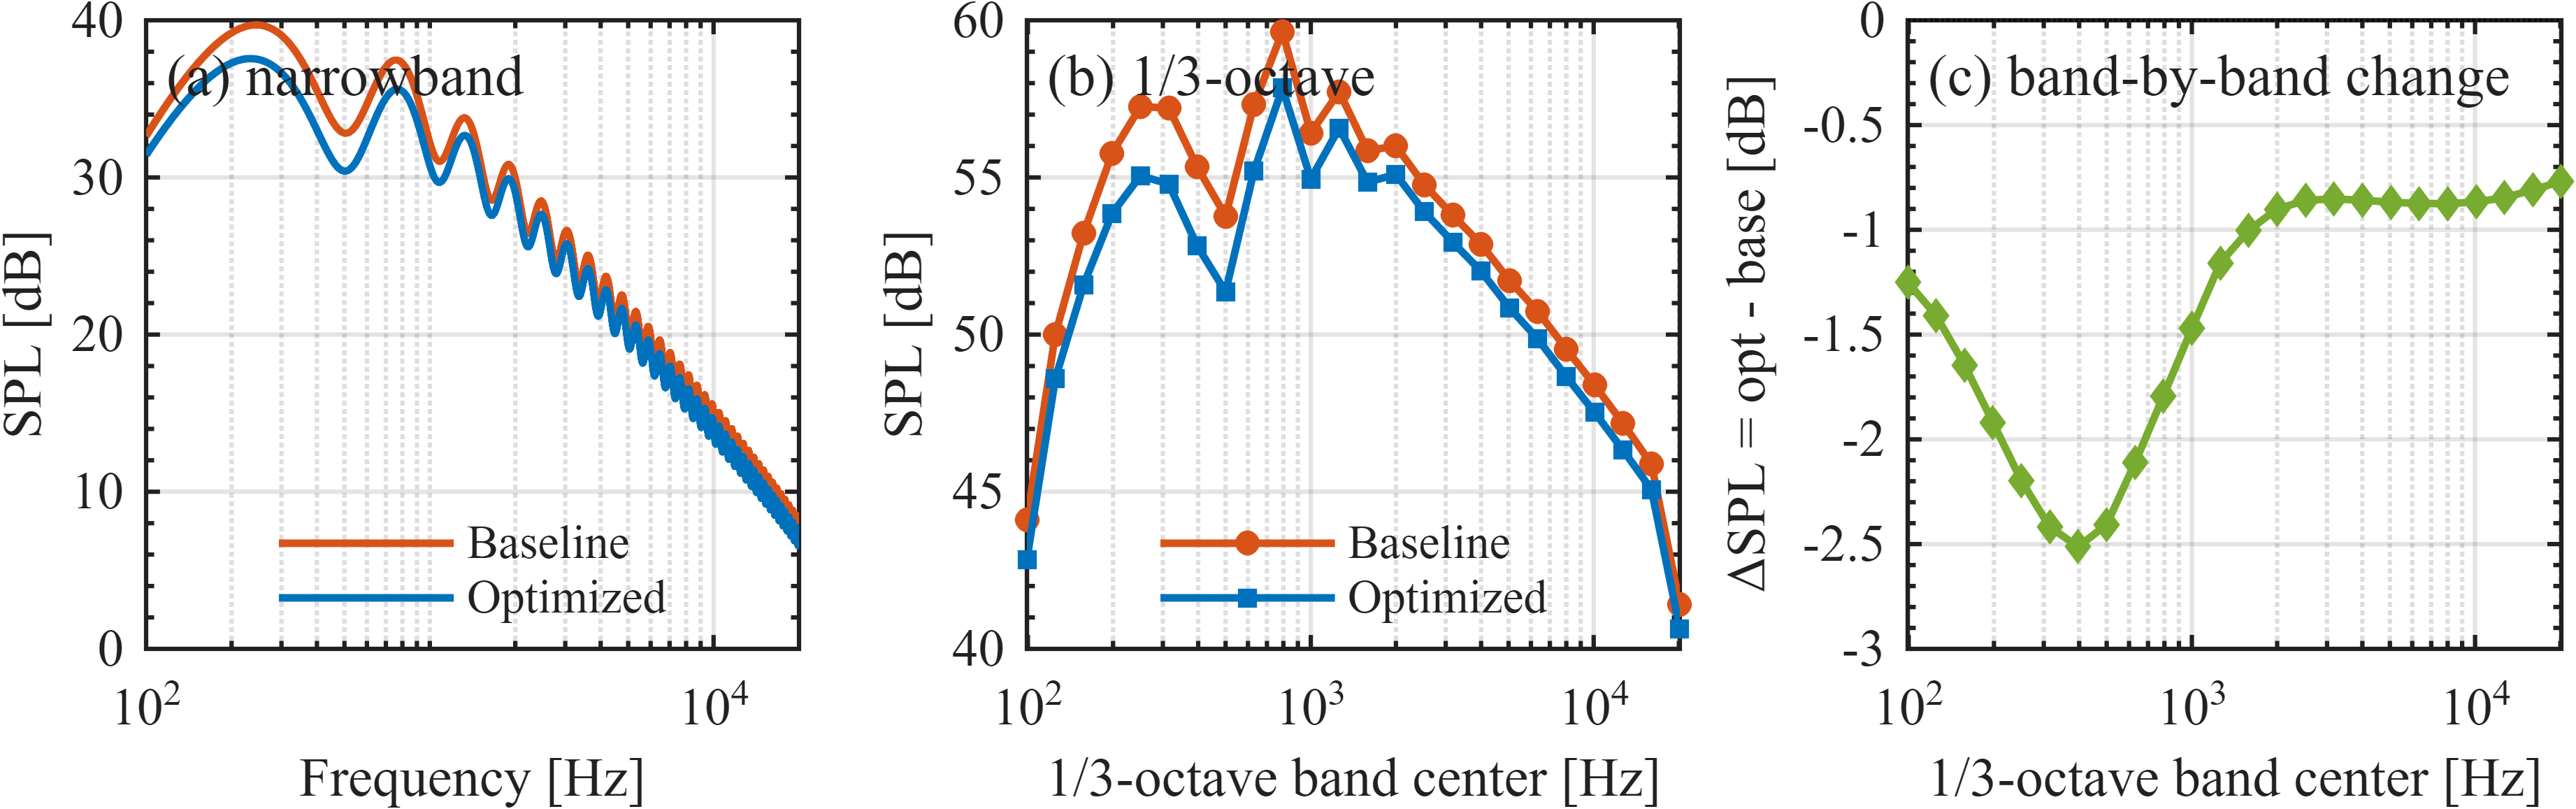
\includegraphics[width=\linewidth]{fig_spectrum_hardcon.png}
\caption{Far-field sound pressure level, baseline versus optimized
($\mathrm{AoA}=\ang{4}$, $Re=3.17\times10^6$, $M=0.24$, observer at \SI{1}{m}):
(left) narrowband, (center) 1/3-octave band, (right) band-by-band change
$\Delta\mathrm{SPL}=\mathrm{SPL}_\mathrm{opt}-\mathrm{SPL}_\mathrm{base}$. The
reduction is largest at low-to-mid frequencies and small at high frequency.}
\label{fig:spec}
\end{figure}

\subsection{Algorithm comparison}\label{sec:algos}
Table~\ref{tab:algo} and Fig.~\ref{fig:algo} compare the five algorithms under
a nominal budget of 150 evaluations starting from the same point. The number
of model calls actually issued varies with the algorithm class
(132--180; population-based methods evaluate in generations and cannot stop
mid-generation), so the comparison is indicative rather than strictly
matched in cost; the reductions below should be read with that caveat.
In these single runs the genetic algorithm reaches the lowest OASPL(A)
(\SI{65.94}{dBA}), followed
closely by surrogate optimization and particle swarm (both
$\approx\SI{66.09}{dBA}$), while pattern search reduces
the noise the least at this small budget (\SI{66.55}{dBA}). The gradient-based
SQP (\SI{66.24}{dBA}) does not stagnate on this constrained problem and, at this
budget, even outperforms pattern search --- the non-smooth, XFOIL-in-the-loop
objective penalizes the local poll of pattern search more than the finite
budget penalizes the population-based methods. The ranking at a fixed small
budget is, however, not the whole story: pattern search, used as the dedicated
single-objective optimizer of the previous subsection, reaches \SI{65.82}{dBA}
at the larger dedicated budget (terminating on mesh tolerance) --- below
\emph{every} solver's 150-evaluation result. The spread between solvers at the
nominal budget ($\approx\SI{0.6}{dBA}$, single runs) is smaller than the gain
obtained from a larger budget ($\approx\SI{0.7}{dBA}$), suggesting that for
this problem the evaluation budget influences the achievable reduction at
least as much as the choice of solver; a statistically matched benchmark
(Section~\ref{sec:concl}) would be needed to separate the two effects
definitively. All methods satisfy the lift-to-drag
constraint and improve
$c_l/c_d$ (to between $56.1$ and $61.3$, the highest found by particle swarm).
The exploration scatter (Fig.~\ref{fig:algo}b) shows how each algorithm samples
the noise--efficiency plane. The fraction of candidates discarded by the penalty
handling (invalid geometry, separated boundary layer or XFOIL non-convergence)
varied between algorithms: $19/151$ for SQP, $21/150$ for surrogate
optimization, $43/134$ for pattern search, $54/132$ for the genetic algorithm
and $103/180$ for particle swarm (the denominator is the total number of XFOIL
evaluations actually performed; population-based methods evaluate in generations
and may exceed or fall short of the nominal 150-evaluation budget). Particle
swarm explores most widely and hits the constraints most often.

Because GA, PSO and SBO are stochastic, the single-run values of
Table~\ref{tab:algo} are not by themselves a reliable ranking. Each was
therefore repeated over 10 independent random seeds at the same nominal
budget (Table~\ref{tab:seeds} and Fig.~\ref{fig:seeds}). The distributions
overlap substantially and, importantly, they \emph{reorder} the single-run
result: over 10 seeds the genetic algorithm is the \emph{least} effective of
the three on average (median \SI{66.20}{dBA}), while particle swarm and
surrogate optimization are marginally better and statistically
indistinguishable from each other (medians \SI{66.02}{} and
\SI{66.01}{dBA}). The single GA run of Table~\ref{tab:algo}
(\SI{65.94}{dBA}) falls below GA's entire 10-seed spread --- i.e.\ it was a
favorable draw rather than evidence that GA is the best solver. The
best single result over all 30 stochastic runs --- \SI{65.65}{dBA}, a
particle-swarm seed --- is in fact the lowest OASPL(A) observed anywhere in
this study, marginally below the pattern-search dedicated optimum of
Section~\ref{sec:opt} (\SI{65.82}{dBA}, mesh-converged at a larger budget).
That seed is not representative of the particle-swarm distribution, however
(its median is \SI{66.02}{dBA}, Table~\ref{tab:seeds}), so it reflects a
favorable draw rather than a systematic advantage of particle swarm over the
budget effect. The deterministic
methods (pattern search and SQP) are seed-independent. The practical
conclusion is that, at this budget, the three stochastic solvers are
equivalent within their seed scatter ($\sigma\le\SI{0.18}{dBA}$), no solver
is a clear winner, and the evaluation budget remains the dominant factor.

\begin{table}[!htbp]\centering
\caption{Ten-seed statistics of the stochastic solvers at the nominal
150-evaluation budget (OASPL(A) in dBA; lower is better). Compare with the
single-run values of Table~\ref{tab:algo}.}
\label{tab:seeds}
\begin{tabular}{@{}lcccccc@{}}
\toprule
Algorithm & median & mean & std & min & max & IQR \\
\midrule
Genetic algorithm      & 66.20 & 66.19 & 0.12 & 66.00 & 66.37 & 0.15 \\
Particle swarm         & 66.02 & 66.01 & 0.18 & \textbf{65.65} & 66.19 & 0.28 \\
Surrogate optimization & 66.01 & 66.02 & 0.10 & 65.88 & 66.17 & 0.20 \\
\bottomrule
\end{tabular}
\end{table}

\begin{figure}[!htbp]\centering
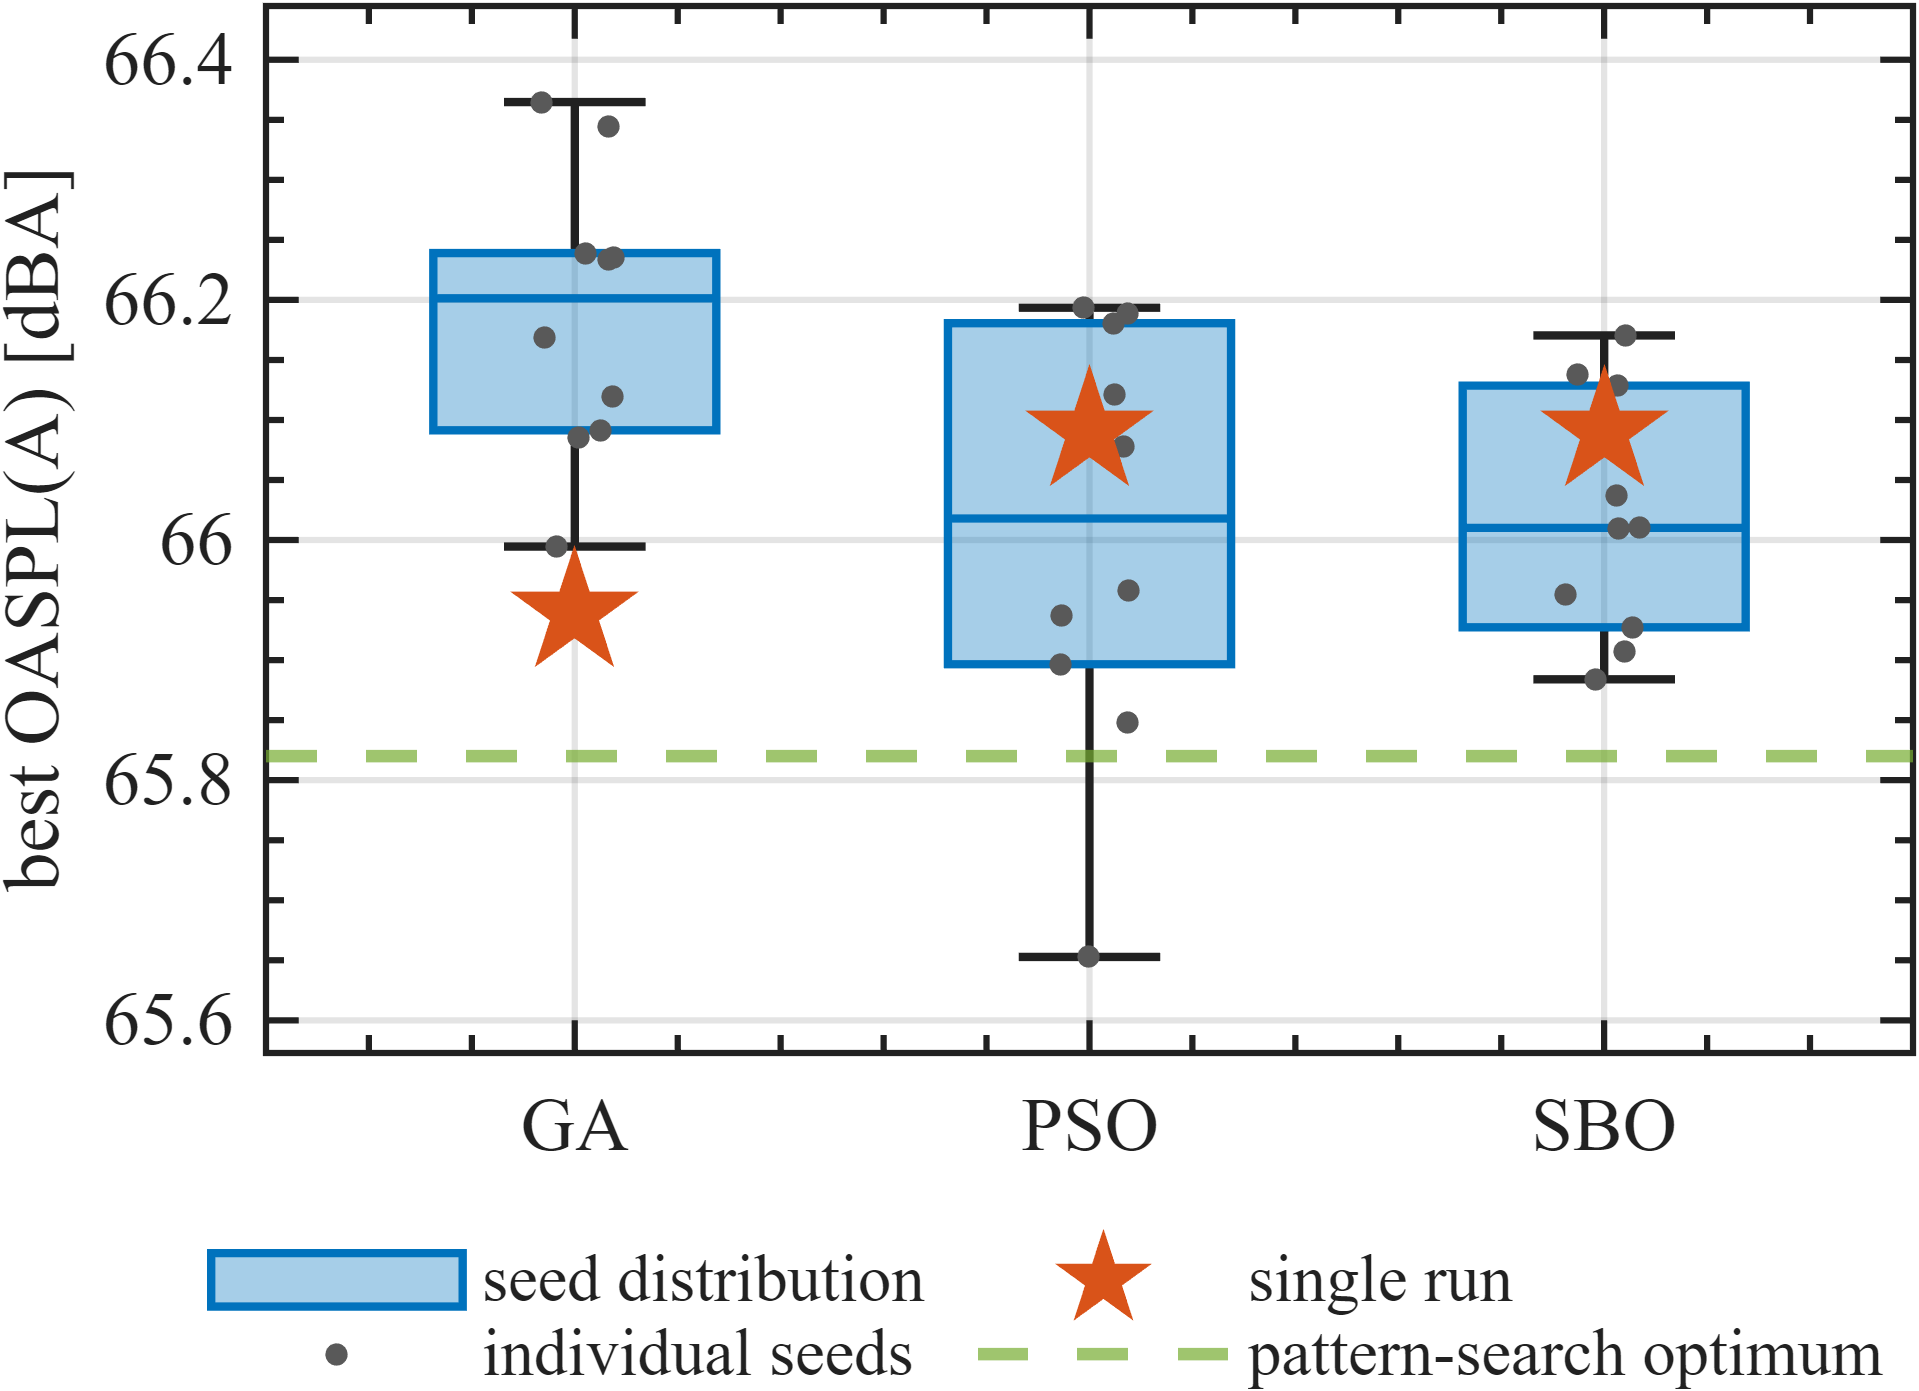
\includegraphics[width=0.62\linewidth]{fig_seed_boxplot.png}
\caption{Distribution of the best OASPL(A) over 10 random seeds for the three
stochastic solvers (box: interquartile range and median; whiskers: extremes;
dots: individual seeds). Orange stars: the single-run values reported in
Table~\ref{tab:algo}; green dashed line: the pattern-search dedicated optimum.
The single GA run lies below GA's full seed distribution.}
\label{fig:seeds}
\end{figure}

\begin{table}[!htbp]\centering
\caption{Best result of each optimization algorithm on the noise-minimization
problem (nominal budget of 150 evaluations; actual calls 132--180, see text).
Baseline OASPL(A) = \SI{67.10}{dBA},
$c_l/c_d = 54.2$. Reductions are computed from unrounded levels; single run
per algorithm.}
\label{tab:algo}
\begin{tabular}{@{}lrrr@{}}
\toprule
Algorithm & OASPL(A) [dBA] & $c_l/c_d$ & Reduction [dBA] \\
\midrule
Genetic algorithm      & \textbf{65.94} & 57.7 & \textbf{1.16} \\
Surrogate optimization & 66.09 & 56.2 & 1.01 \\
Particle swarm         & 66.09 & 61.3 & 1.00 \\
SQP (gradient)         & 66.24 & 57.3 & 0.85 \\
Pattern search         & 66.55 & 56.1 & 0.55 \\
\bottomrule
\end{tabular}
\end{table}

\begin{figure}[!htbp]\centering
\begin{subfigure}{0.48\linewidth}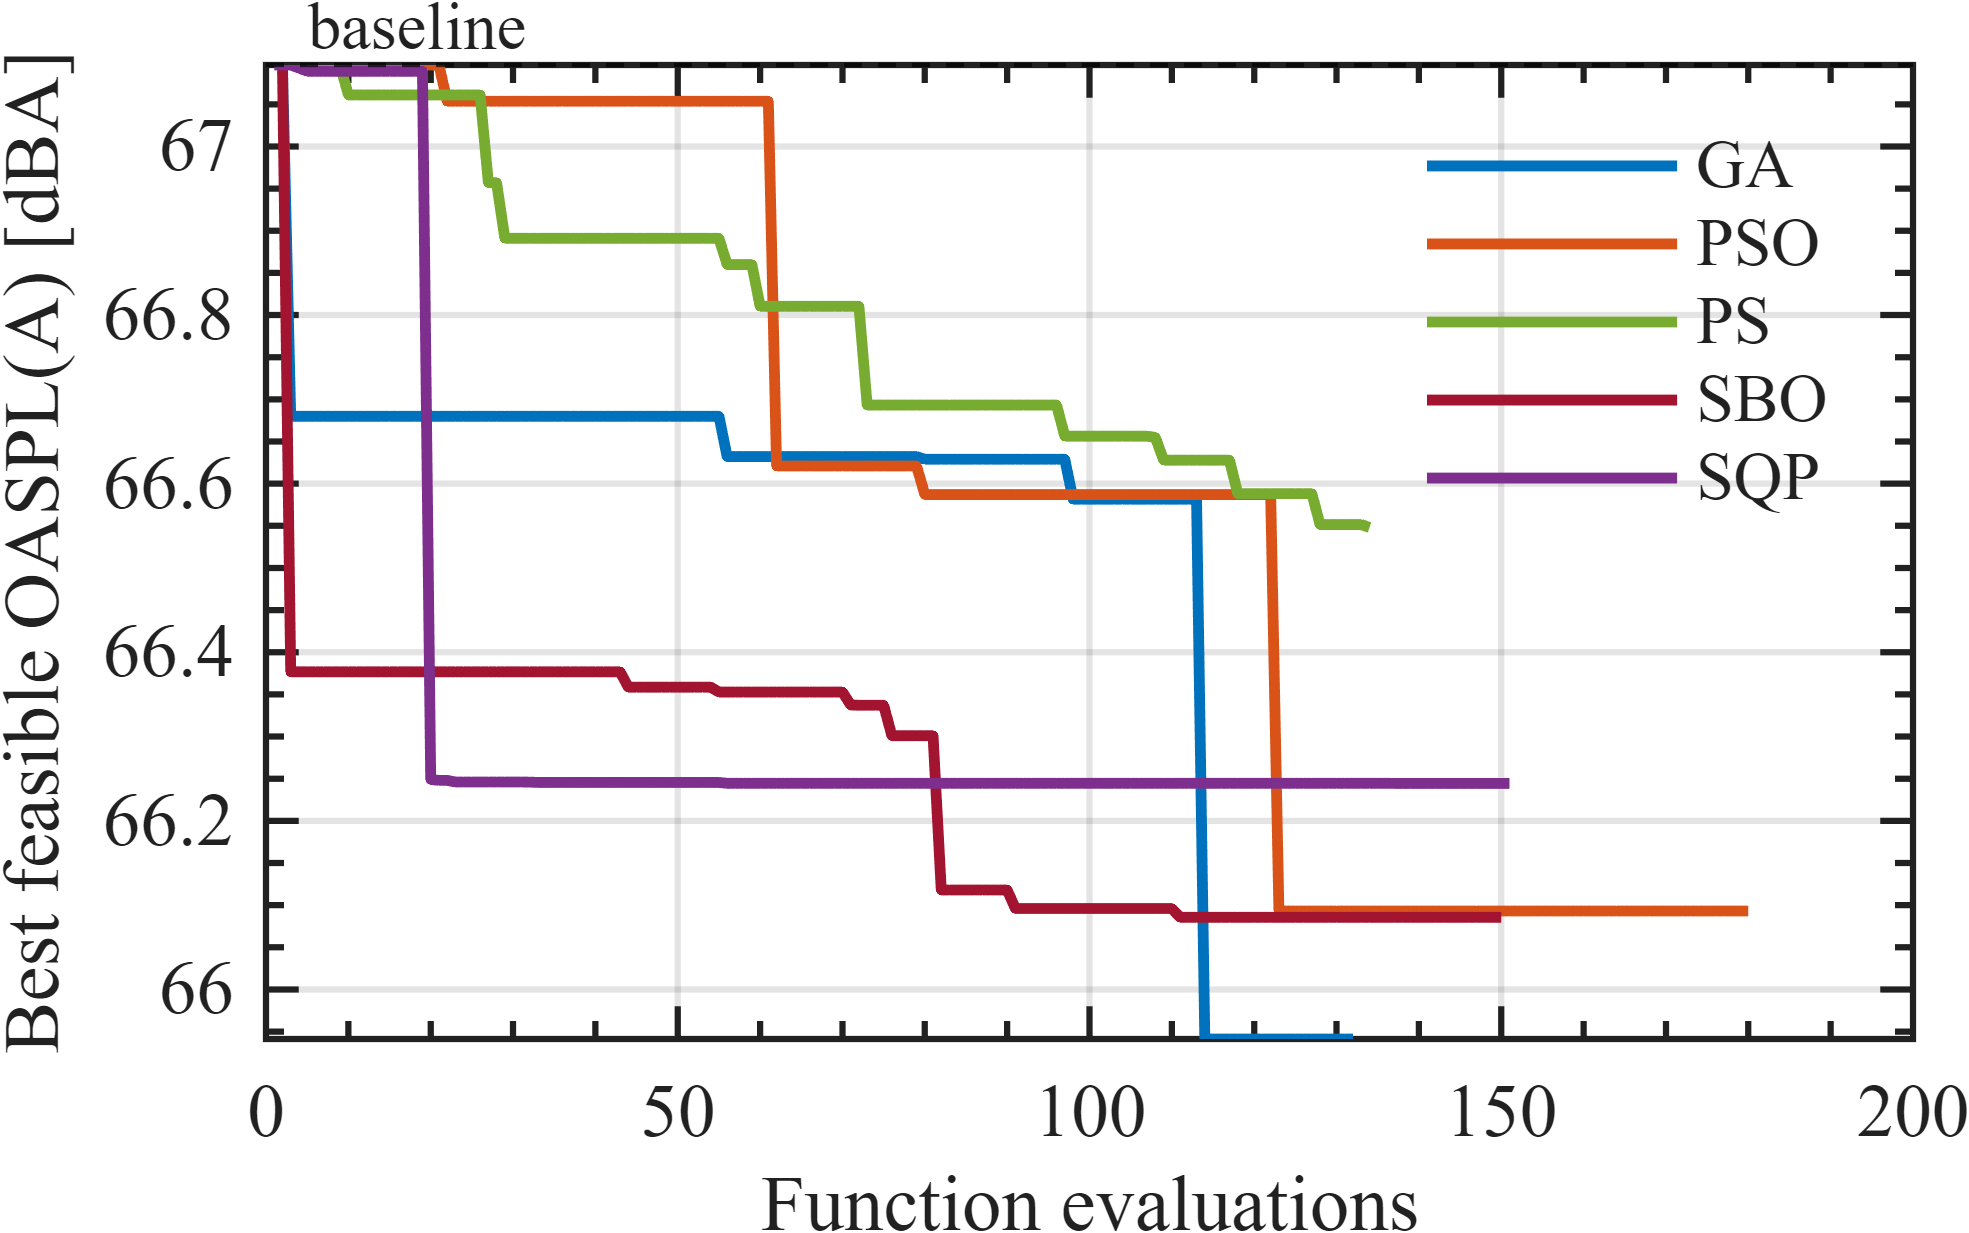
\includegraphics[width=\linewidth]{fig_algo_convergence.png}
\caption{}\end{subfigure}\hfill
\begin{subfigure}{0.48\linewidth}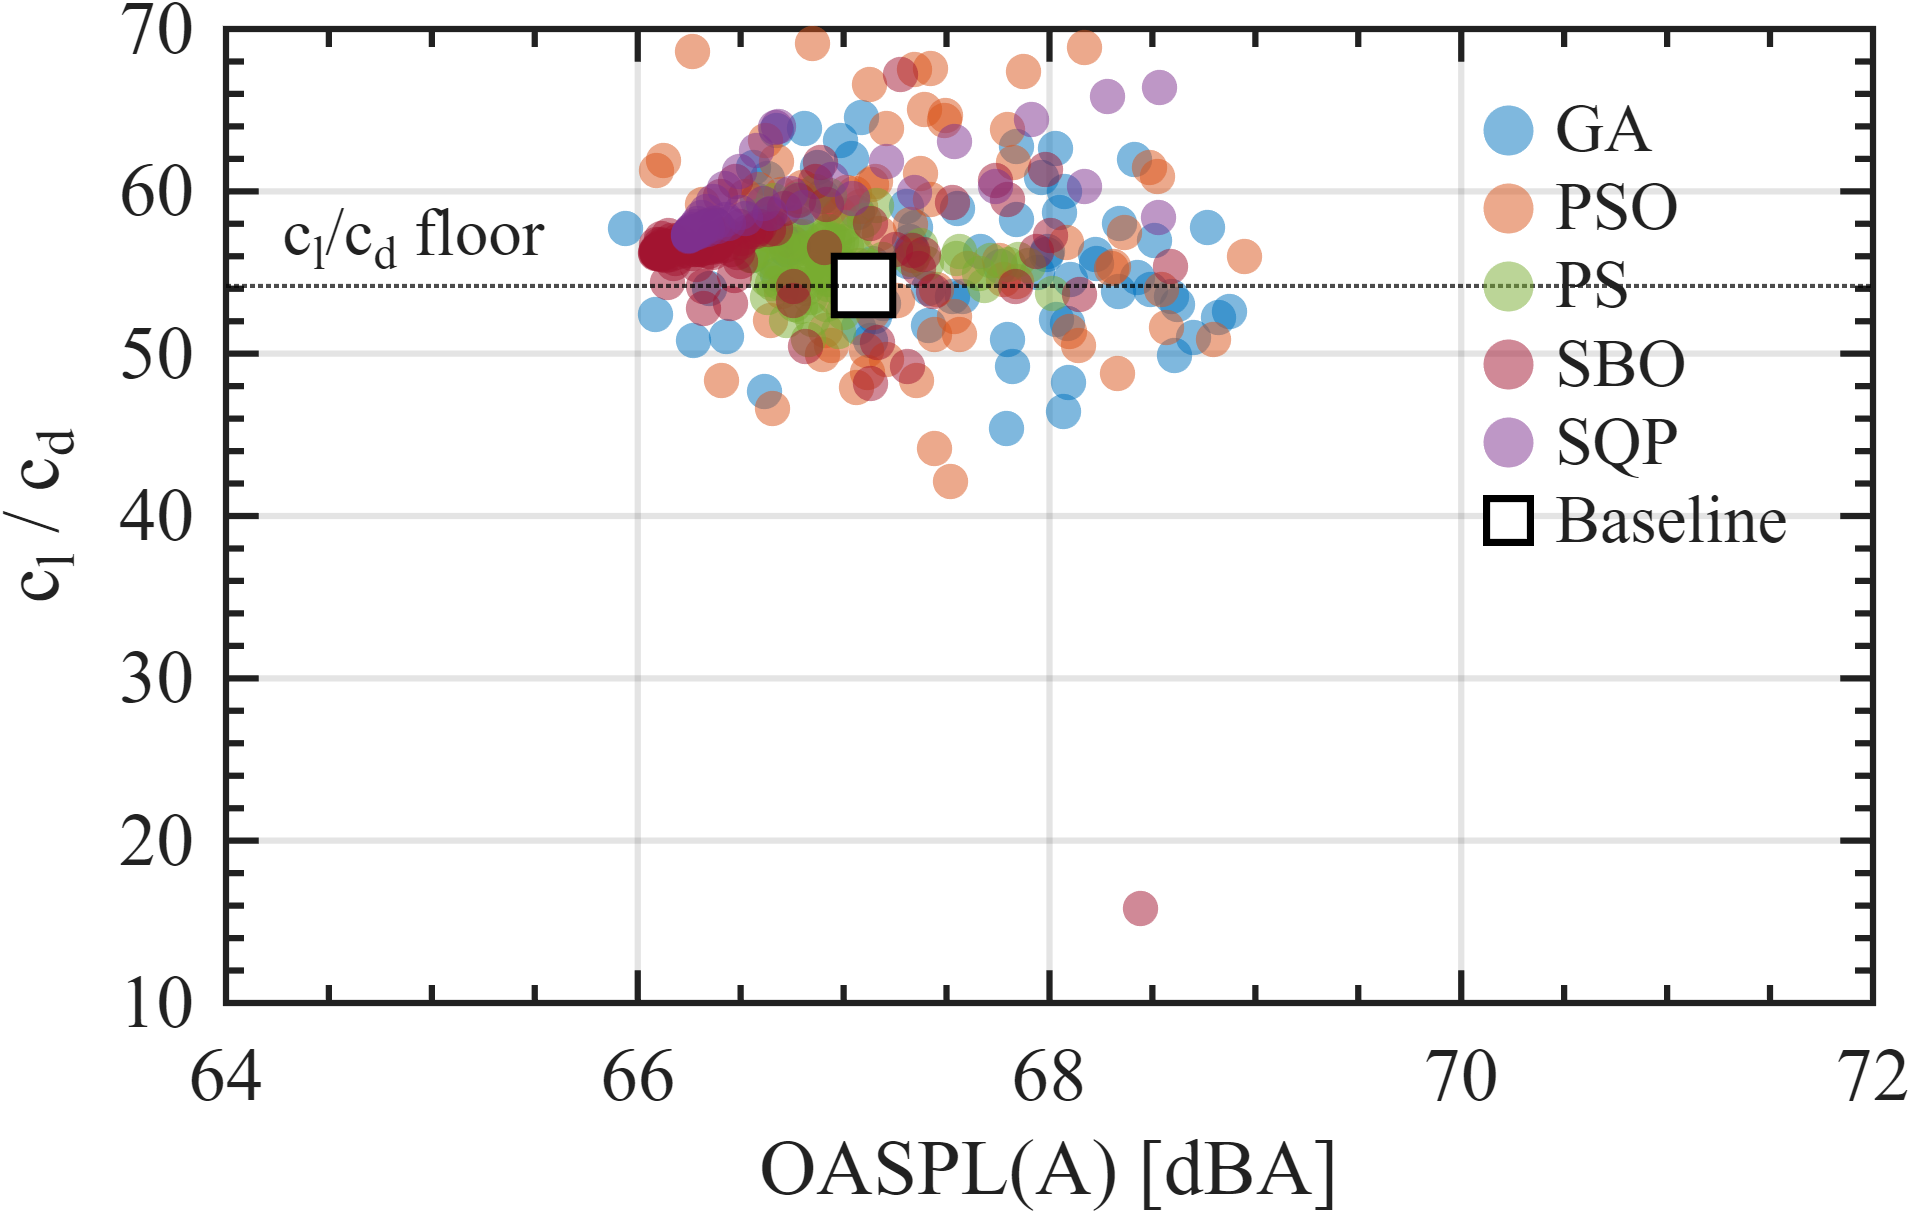
\includegraphics[width=\linewidth]{fig_algo_exploration.png}
\caption{}\end{subfigure}
\caption{(a) Convergence history of the five optimizers. (b) Designs explored
by each optimizer in the noise--efficiency plane (axis focused on the feasible
cloud; a few discarded candidates lie at higher OASPL).}
\label{fig:algo}
\end{figure}

\subsection{Pareto front}\label{sec:pareto}
The multi-objective optimization (\texttt{gamultiobj}, population 40 over 30
generations, i.e.\ up to 1200 evaluations, yielding a final non-dominated set
of 40 designs; Fig.~\ref{fig:pareto}) maps the trade-off
between noise and aerodynamic efficiency, providing a family of designs rather
than a single optimum and quantifying the noise penalty of demanding higher
$c_l/c_d$. The front is used qualitatively, to establish dominance over the
baseline and the efficiency-unconstrained noise floor, rather than as a
converged Pareto set (no hypervolume convergence criterion was imposed). All three representative designs of Table~\ref{tab:pareto}
\emph{dominate} the baseline (lower OASPL \emph{and} higher $c_l/c_d$): the
baseline is dominated by several designs found within the explored CST design
space, and noise can be reduced without sacrificing
efficiency. The three designs are somewhat thinner than the baseline
($t_{\max}/c$ between $0.178$ and $0.184$ versus $0.210$) and considerably more
cambered, raising the efficiency to $c_l/c_d=72$--$74$ against $54.2$ at noise
levels between \SI{65.96}{dBA} (minimum-noise) and \SI{66.59}{dBA}
(maximum-efficiency, still \SI{0.5}{dBA} below the baseline). Notably, the
minimum-noise design approaches the level of the single-objective optimum
(\SI{65.96}{dBA} against \SI{65.82}{dBA}) even though it does not enforce the
lift-to-drag constraint, corroborating that within the chosen design box the
constrained optimum is not a constraint artefact.

\begin{table}[!htbp]\centering
\caption{Representative Pareto designs (minimum-noise, intermediate,
maximum-efficiency) compared with the baseline.}
\label{tab:pareto}
\begin{tabular}{@{}lrrrrrr@{}}
\toprule
Design & OASPL(A) [dBA] & $c_l$ & $c_d$ & $c_l/c_d$ & $t_{\max}/c$ & $c_m$ \\
\midrule
\textbf{baseline} & 67.10 & 0.630 & 0.0116 & 54.2 & 0.210 & $-0.038$ \\
min-noise         & 65.96 & 0.866 & 0.0120 & 72.3 & 0.184 & $-0.075$ \\
intermediate      & 66.18 & 0.868 & 0.0119 & 72.7 & 0.184 & $-0.075$ \\
max-efficiency    & 66.59 & 0.861 & 0.0117 & 73.7 & 0.178 & $-0.069$ \\
\bottomrule
\end{tabular}
\end{table}

\begin{figure}[!htbp]\centering
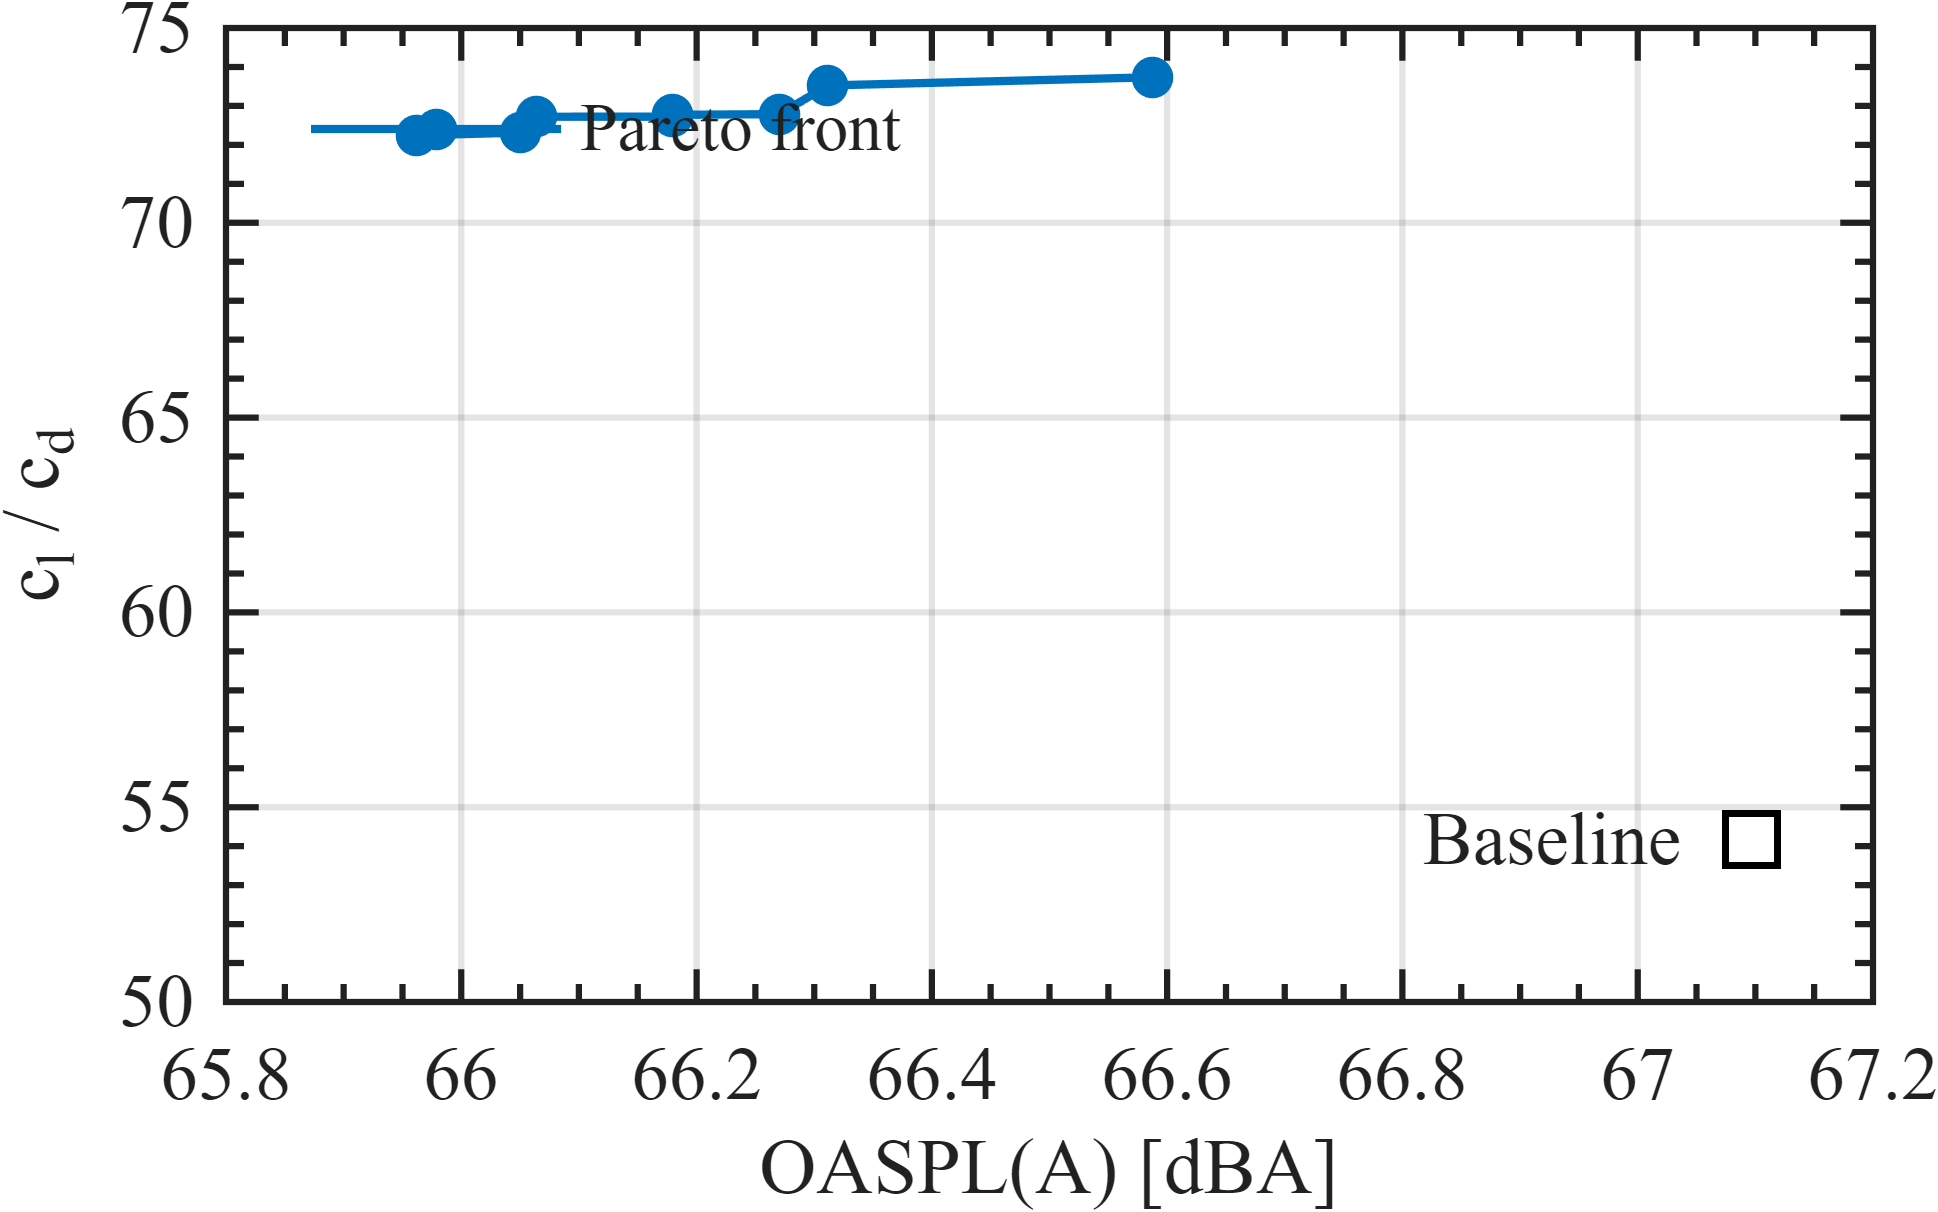
\includegraphics[width=0.7\linewidth]{fig_pareto_front.png}
\caption{Pareto front: A-weighted OASPL versus lift-to-drag ratio.}
\label{fig:pareto}
\end{figure}

\subsection{Robust multi-model optimization of the NACA 63-218}\label{sec:63218}
To test the generality of the framework and to address the wall-pressure
model-form uncertainty documented in Section~\ref{sec:sens}, the
\SI{18}{\percent} section of the same family (NACA 63-218; baseline
OASPL(A) $=\SI{67.82}{dBA}$, $c_l/c_d=60.1$ at the same operating point) was
optimized with a \emph{robust multi-model} objective. Instead of minimizing the
noise predicted by a single wall-pressure model, the objective minimizes the
\emph{worst case} among the three wall-pressure models available in the
prediction chain (TNO--Blake, Goody and Kamruzzaman),
\begin{equation}
\min_{\mathbf a}\ \max\!\bigl[\mathrm{OASPL(A)}_\mathrm{TNO},\,
\mathrm{OASPL(A)}_\mathrm{Goody},\,
\mathrm{OASPL(A)}_\mathrm{Kamr}\bigr](\mathbf a),
\label{eq:robust}
\end{equation}
This worst-case objective [Eq.~\eqref{eq:robust}] is subject to the same
aerodynamic and geometric constraints as the main case
[Eq.~\eqref{eq:problem}]. To give the search enough freedom to reshape the
section, the design box is widened to $\pm80\%$ of the baseline
coefficients and the thickness cap is relaxed to $1.4\,T_0$; the run uses the
dedicated single-objective budget of 2000 evaluations and converged on the
$10^{-4}$ mesh tolerance after 1293 calls. Table~\ref{tab:63218} and
Fig.~\ref{fig:63218} summarize the robust optimum.

\begin{table}[!htbp]\centering
\caption{NACA 63-218 robust optimum: OASPL(A) [dBA] re-evaluated with the three
wall-pressure models used in the worst-case objective,
compared with the baseline. The optimum lowers all three models simultaneously
while improving the lift-to-drag ratio and preserving the maximum thickness.
Robust run: min--max over TNO/Goody/Kamruzzaman, expanded $\pm80\%$ box,
dedicated 2000-evaluation budget (mesh-converged in 1293 calls).}
\label{tab:63218}
\begin{tabular}{@{}lccccc@{}}
\toprule
Design & TNO & Goody & Kamruzzaman & $c_l/c_d$ & $t_{\max}/c$ \\
\midrule
baseline                & 67.82 & 64.08 & 67.45 & 60.1 & 0.181 \\
\textbf{robust optimum} & \textbf{65.64} & \textbf{62.04} & \textbf{65.54} & \textbf{63.2} & 0.180 \\
\midrule
reduction               & $2.18$ & $2.04$ & $1.91$ & $+3.1$ & --- \\
\bottomrule
\end{tabular}
\end{table}

\begin{figure}[!htbp]\centering
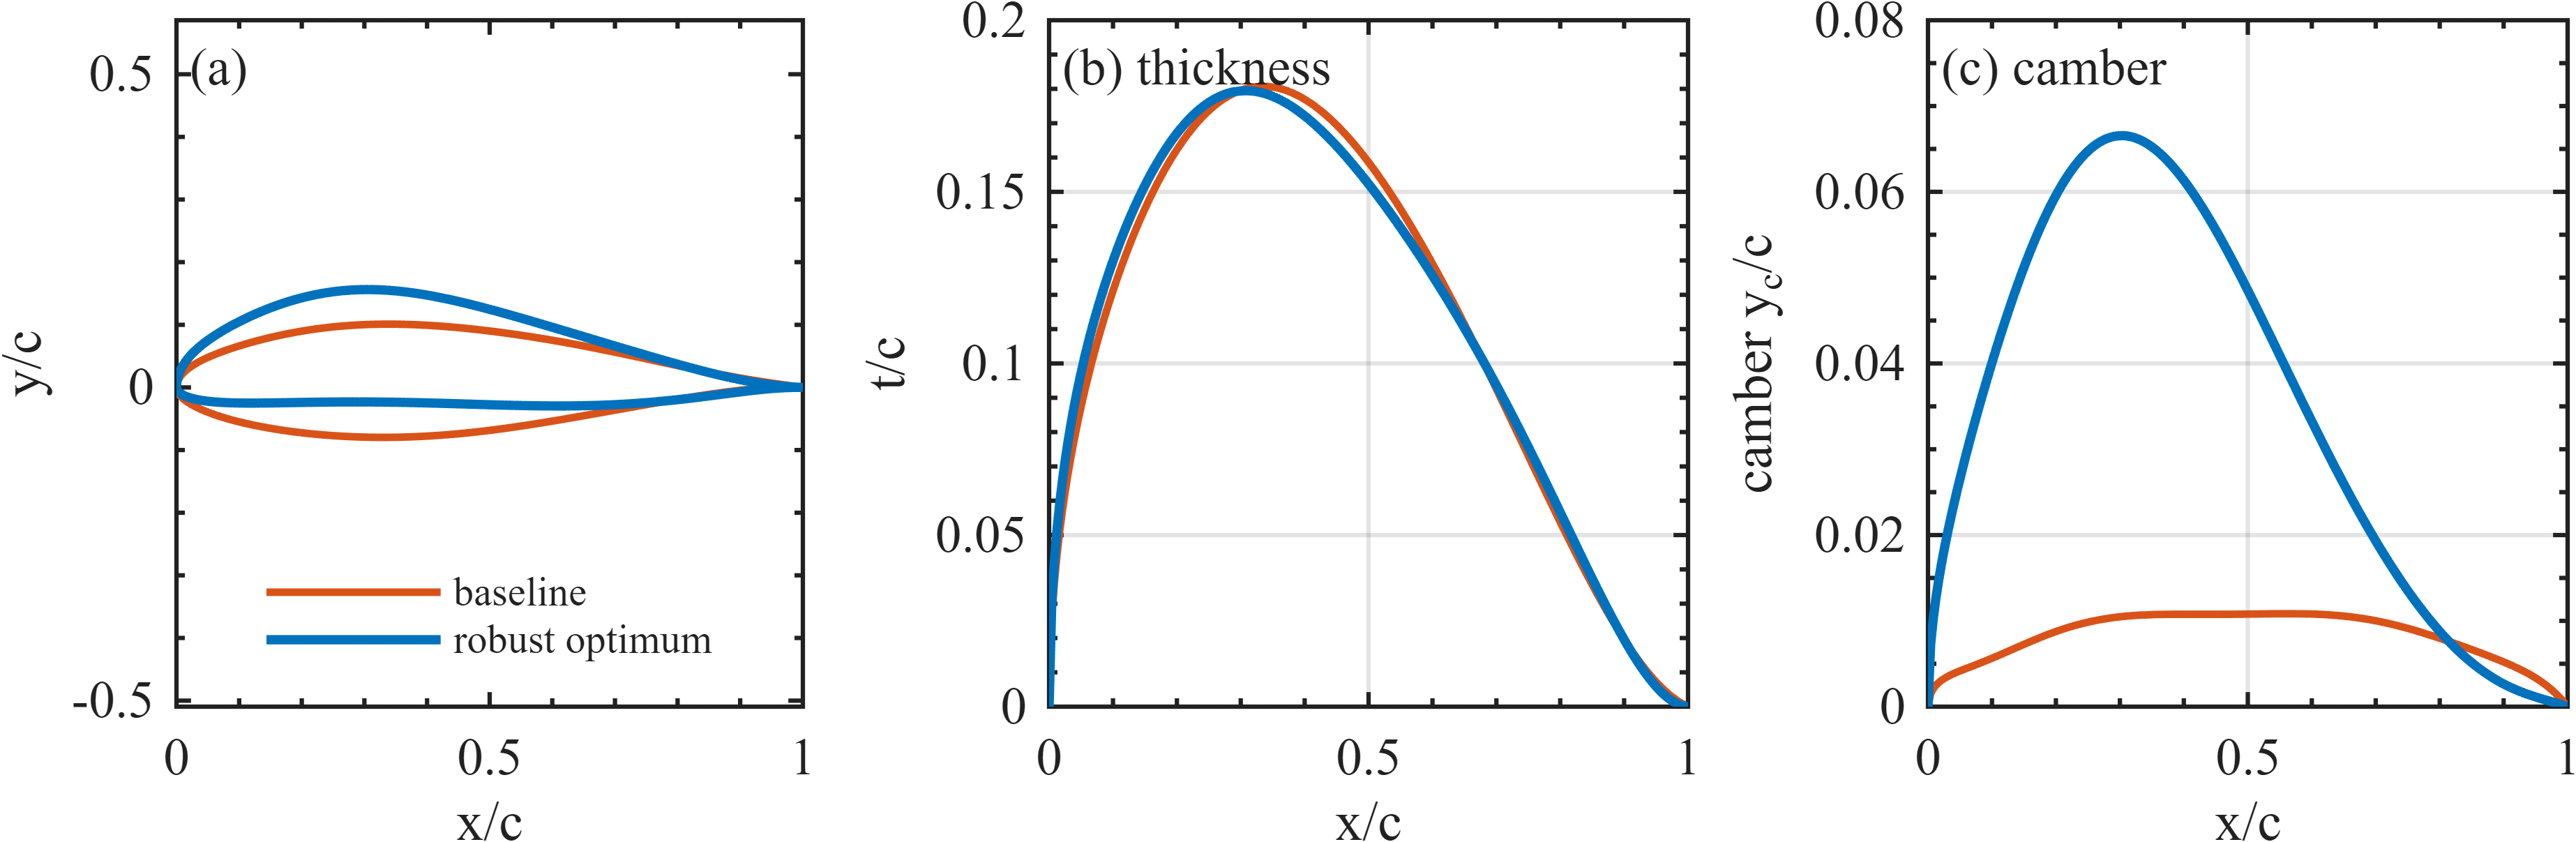
\includegraphics[width=\linewidth]{fig_63218_geometry.png}
\caption{NACA 63-218 robust optimum (orange: baseline, blue: robust optimum):
(a) silhouettes, (b) thickness distribution, (c) camber line. The optimum
preserves the maximum thickness ($\approx\SI{18}{\percent}$) and reshapes the
section by adding forward camber --- the same constant-thickness mechanism as
the 63-221 case.}
\label{fig:63218}
\end{figure}

Two results stand out. First, the robust optimum lowers the predicted noise in
\emph{all three} wall-pressure models simultaneously --- by
\SI{2.18}{dBA} (TNO), \SI{2.04}{dBA} (Goody) and \SI{1.91}{dBA}
(Kamruzzaman) --- so the reduction is consistent across the three models
assessed here rather than conditional on the choice of a single wall-pressure
model. Second, the geometric mechanism is the \emph{same} as in the 63-221 main
case: the robust optimum keeps the maximum thickness at
essentially the baseline value ($t_{\max}/c$: $0.181\!\to\!0.180$, the relaxed
cap remaining inactive) and reshapes the section by adding forward camber
(maximum camber $0.011\!\to\!0.067$, its location moving from
$x/c\approx0.56$ to $0.31$; Fig.~\ref{fig:63218}). The added camber raises the
lift-to-drag ratio from $60.1$ to $63.2$, so the robust optimum
\emph{dominates} the baseline --- quieter across the three models and
aerodynamically more efficient --- while preserving an approximately
\SI{18}{\percent} maximum thickness.

The robust optimum was subsequently re-evaluated through a separate XFOIL polar
sweep, independent of the optimization loop although not of the aerodynamic
model itself. The sweep reproduces the design-point $c_l/c_d=63.2$ and, being a
conventional \SI{18}{\percent} section, converges over the usual operating
range with an attached boundary layer; its off-design acoustic behavior, and
the reduced negative-incidence margin introduced by the added camber, are
examined in Section~\ref{sec:sens}.

Because the worst-case objective [Eq.~\eqref{eq:robust}] compares \emph{absolute}
levels, and the three models differ in baseline offset (\SI{67.8}{}, \SI{64.1}{}
and \SI{67.4}{dBA} for TNO, Goody and Kamruzzaman), it could in principle be
driven by the model with the highest offset rather than by the largest
geometric improvement. As a check, the 63-218 was re-optimized with a
\emph{relative} worst-case objective that refers each model to its own baseline,
\begin{equation}
\min_{\mathbf a}\ \max_m\bigl[\,L_m(\mathbf a)-L_m(\mathbf a_0)\,\bigr],
\qquad m\in\{\mathrm{TNO,\ Goody,\ Kamruzzaman}\},
\label{eq:robustrel}
\end{equation}
i.e.\ minimizing the worst \emph{change} relative to the baseline
[Eq.~\eqref{eq:robustrel}] (equivalently, maximizing the smallest per-model
reduction). Under the same domain, constraints
and budget, this yields a very similar conventional section
(\SI{17}{\percent} maximum thickness, $c_l/c_d=63.2$) that again reduces all
three models, with a slightly better balance: the per-model reductions become
\SI{2.2}{}, \SI{3.0}{} and \SI{2.4}{dBA} (TNO, Goody, Kamruzzaman), raising the
\emph{smallest} of the three from the \SI{1.9}{dBA} of the absolute-objective
optimum (Table~\ref{tab:63218}, Kamruzzaman-limited) to \SI{2.2}{dBA}. The two
optima are otherwise equivalent, so the absolute-objective optimum of
Table~\ref{tab:63218} is retained as the reported design; the relative
formulation confirms that the reported reduction is a genuine geometric
improvement shared by the three models, not an artefact of their differing
absolute offsets.

\subsection{Model sensitivity and off-design behavior}\label{sec:sens}
Two additional checks quantify how far the predicted reductions can be
trusted. First, the optimized 63-221 geometry (obtained with the TNO model) was
re-evaluated \emph{post hoc} with two alternative wall-pressure models
available in the prediction chain, Goody \citep{Goody2004} and Kamruzzaman
\citep{Kamruzzaman2015}, without re-optimizing (Table~\ref{tab:wps}). The
outcome reveals substantial model-form uncertainty. The Goody model predicts
comparable (indeed larger) reductions; however, Goody was developed
primarily for near-zero-pressure-gradient boundary layers, so its agreement
cannot be read as an independent confirmation in a problem where the adverse
pressure gradient is central. The Kamruzzaman model, which explicitly
incorporates pressure-gradient and loading effects, does \emph{not} confirm
the benefit of this \emph{single-model} optimum: it reverses the reduction
(Table~\ref{tab:wps}). Figure~\ref{fig:wpsdelta} locates the disagreement: at
mid-to-high frequencies all three models predict a quieter suction side, but
Kamruzzaman predicts \emph{increases} where the other two predict decreases
--- uniformly (\SIrange{1.6}{1.9}{dB}) on the pressure side, the dominant
source of this thick section, and below $\approx\SI{400}{Hz}$ on the suction
side --- consistent with its stronger penalization of the optimum's
increased aft loading through the pressure-gradient term. For a single-model
optimum the predicted decibel figures are therefore comparable to the
wall-pressure model-form uncertainty and should be read within the TNO
framework in which they were obtained --- the model that was assessed against
reference data in Section~\ref{sec:noise}. This sensitivity is precisely what
motivated the robust multi-model optimization of Section~\ref{sec:63218}: its
NACA 63-218 optimum lowers the noise in \emph{all three} wall-pressure
models simultaneously (\SIrange{1.9}{2.2}{dBA}, Table~\ref{tab:63218}), so the
predicted benefit is consistent across the three wall-pressure models
considered rather than conditional on any single one. For
the single-model 63-221 optimum, a per-model or robust re-optimization and
higher-fidelity (RANS/LES or experimental) confirmation remain necessary
before hardware decisions.

\begin{figure}[!htbp]\centering
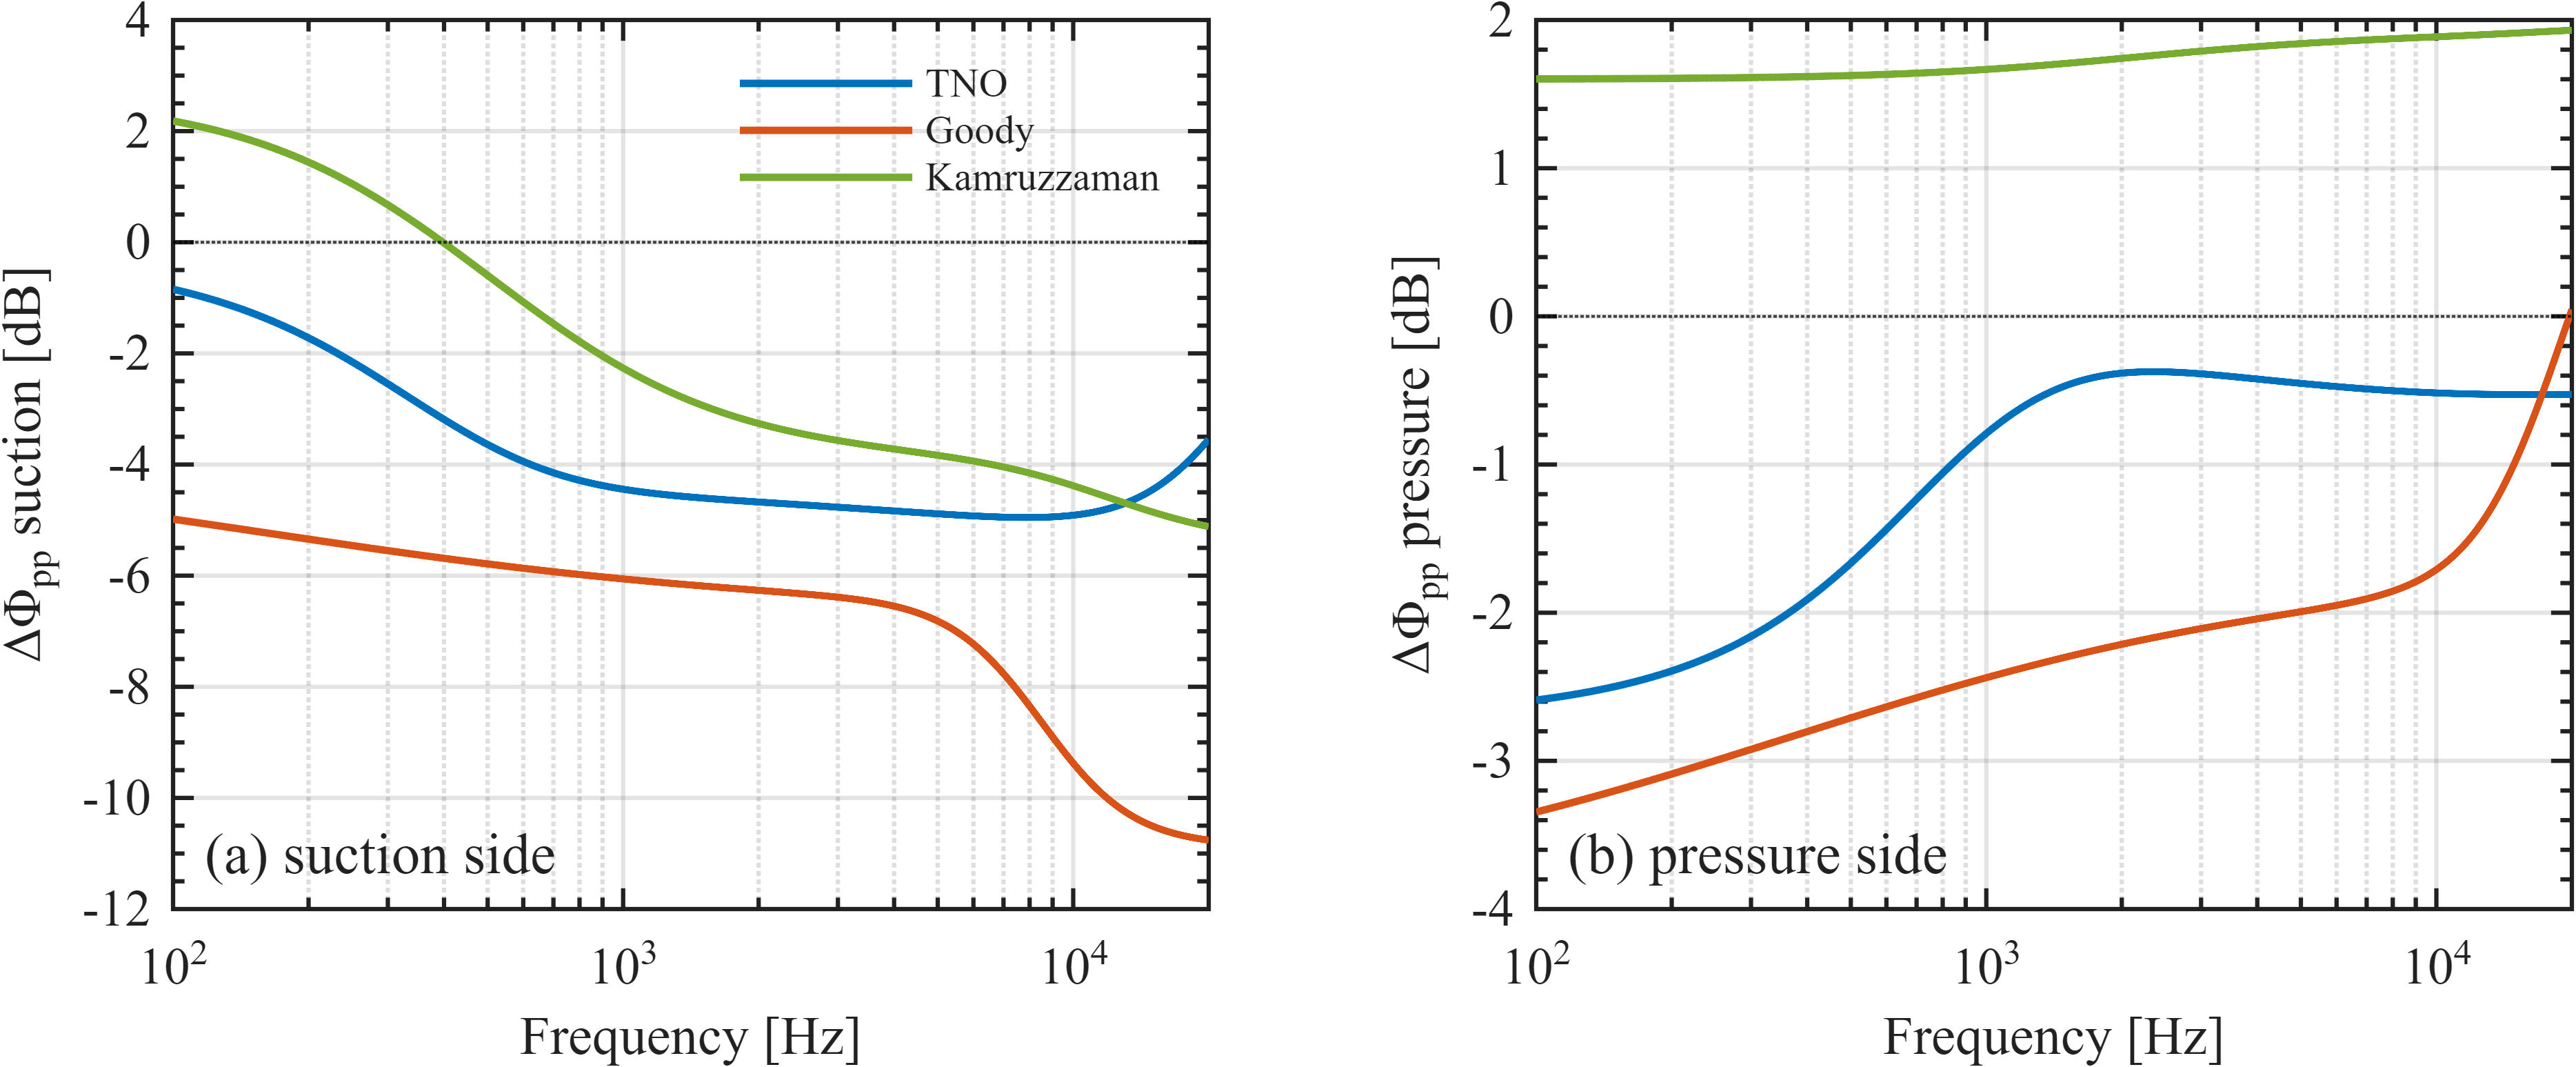
\includegraphics[width=\linewidth]{fig_wps_delta_NACA63221.png}
\caption{Change of the wall-pressure spectrum at $x/c=0.99$ produced by the
63-221 optimization ($\Delta\Phi_{pp}$ = optimum $-$ baseline) as predicted
by each wall-pressure model: (a) suction side, (b) pressure side.}
\label{fig:wpsdelta}
\end{figure}

\begin{table}[!htbp]\centering
\caption{Model-form sensitivity of the single-model NACA 63-221 optimum:
OASPL(A) [dBA] of the baseline and the TNO-obtained optimum re-evaluated with
each wall-pressure model (no re-optimization). $\Delta =
L_{\mathrm{base}}-L_{\mathrm{opt}}$, positive when the optimum is quieter. The
Kamruzzaman model does not confirm the single-model reduction, which motivated
the robust multi-model optimization of the 63-218 (Table~\ref{tab:63218}).}
\label{tab:wps}
\begin{tabular}{@{}lccc@{}}
\toprule
Model & base & optimum & $\Delta$ \\
\midrule
TNO--Blake  & 67.10 & 65.82 & $1.28$ \\
Goody       & 63.21 & 60.82 & $2.39$ \\
Kamruzzaman & 66.03 & 66.71 & $-0.68$ \\
\bottomrule
\end{tabular}
\end{table}

Second, both optima were re-evaluated off-design at two flow conditions
(Fig.~\ref{fig:offdesign}); the robust 63-218 optimum was additionally swept
down to negative incidence. The Reynolds number was
varied through the inflow velocity at constant $\nu=1.5\times10^{-5}$~m$^2$/s
and fixed trip location: $U_\infty=\SI{83.31}{m/s}$ gives
$Re=3.17\times10^6$, $M=0.24$, and $U_\infty=\SI{60.0}{m/s}$ gives
$Re=2.28\times10^6$, $M=0.17$; Mach therefore co-varies with Reynolds, and an
independent Mach variation was not performed. The robust 63-218 optimum retains
\SIrange{1.2}{2.2}{dBA} of reduction over $\alpha=2$--$6^{\circ}$ at both
conditions, peaking at \SI{2.2}{dBA} at the design point; because of its high
forward camber, however, the benefit diminishes toward low incidence and
\emph{reverses} at negative angles --- the optimum becomes up to \SI{1.3}{dBA}
\emph{louder} for $\alpha\le-6^{\circ}$ --- as the cambered section approaches
its lower-surface (negative-incidence) stall. This reduced negative-incidence
margin must be checked against gust and negative-$\alpha$ requirements before
use on a blade. The 63-221 optimum retains
\SIrange{1.1}{1.3}{dBA} for $\alpha=2$--$5^{\circ}$ at both conditions
but loses most of its margin at $\alpha=6^{\circ}$, where this thick section
approaches its attachment limit --- consistent with the design-point choice
of Section~\ref{sec:opt}. Because the Reynolds number was changed through the
inflow velocity, Mach co-varied with it and its independent effect was not
isolated; roughness and inflow-turbulence
variations remain untested.

\begin{figure}[!htbp]\centering
\begin{subfigure}{0.48\linewidth}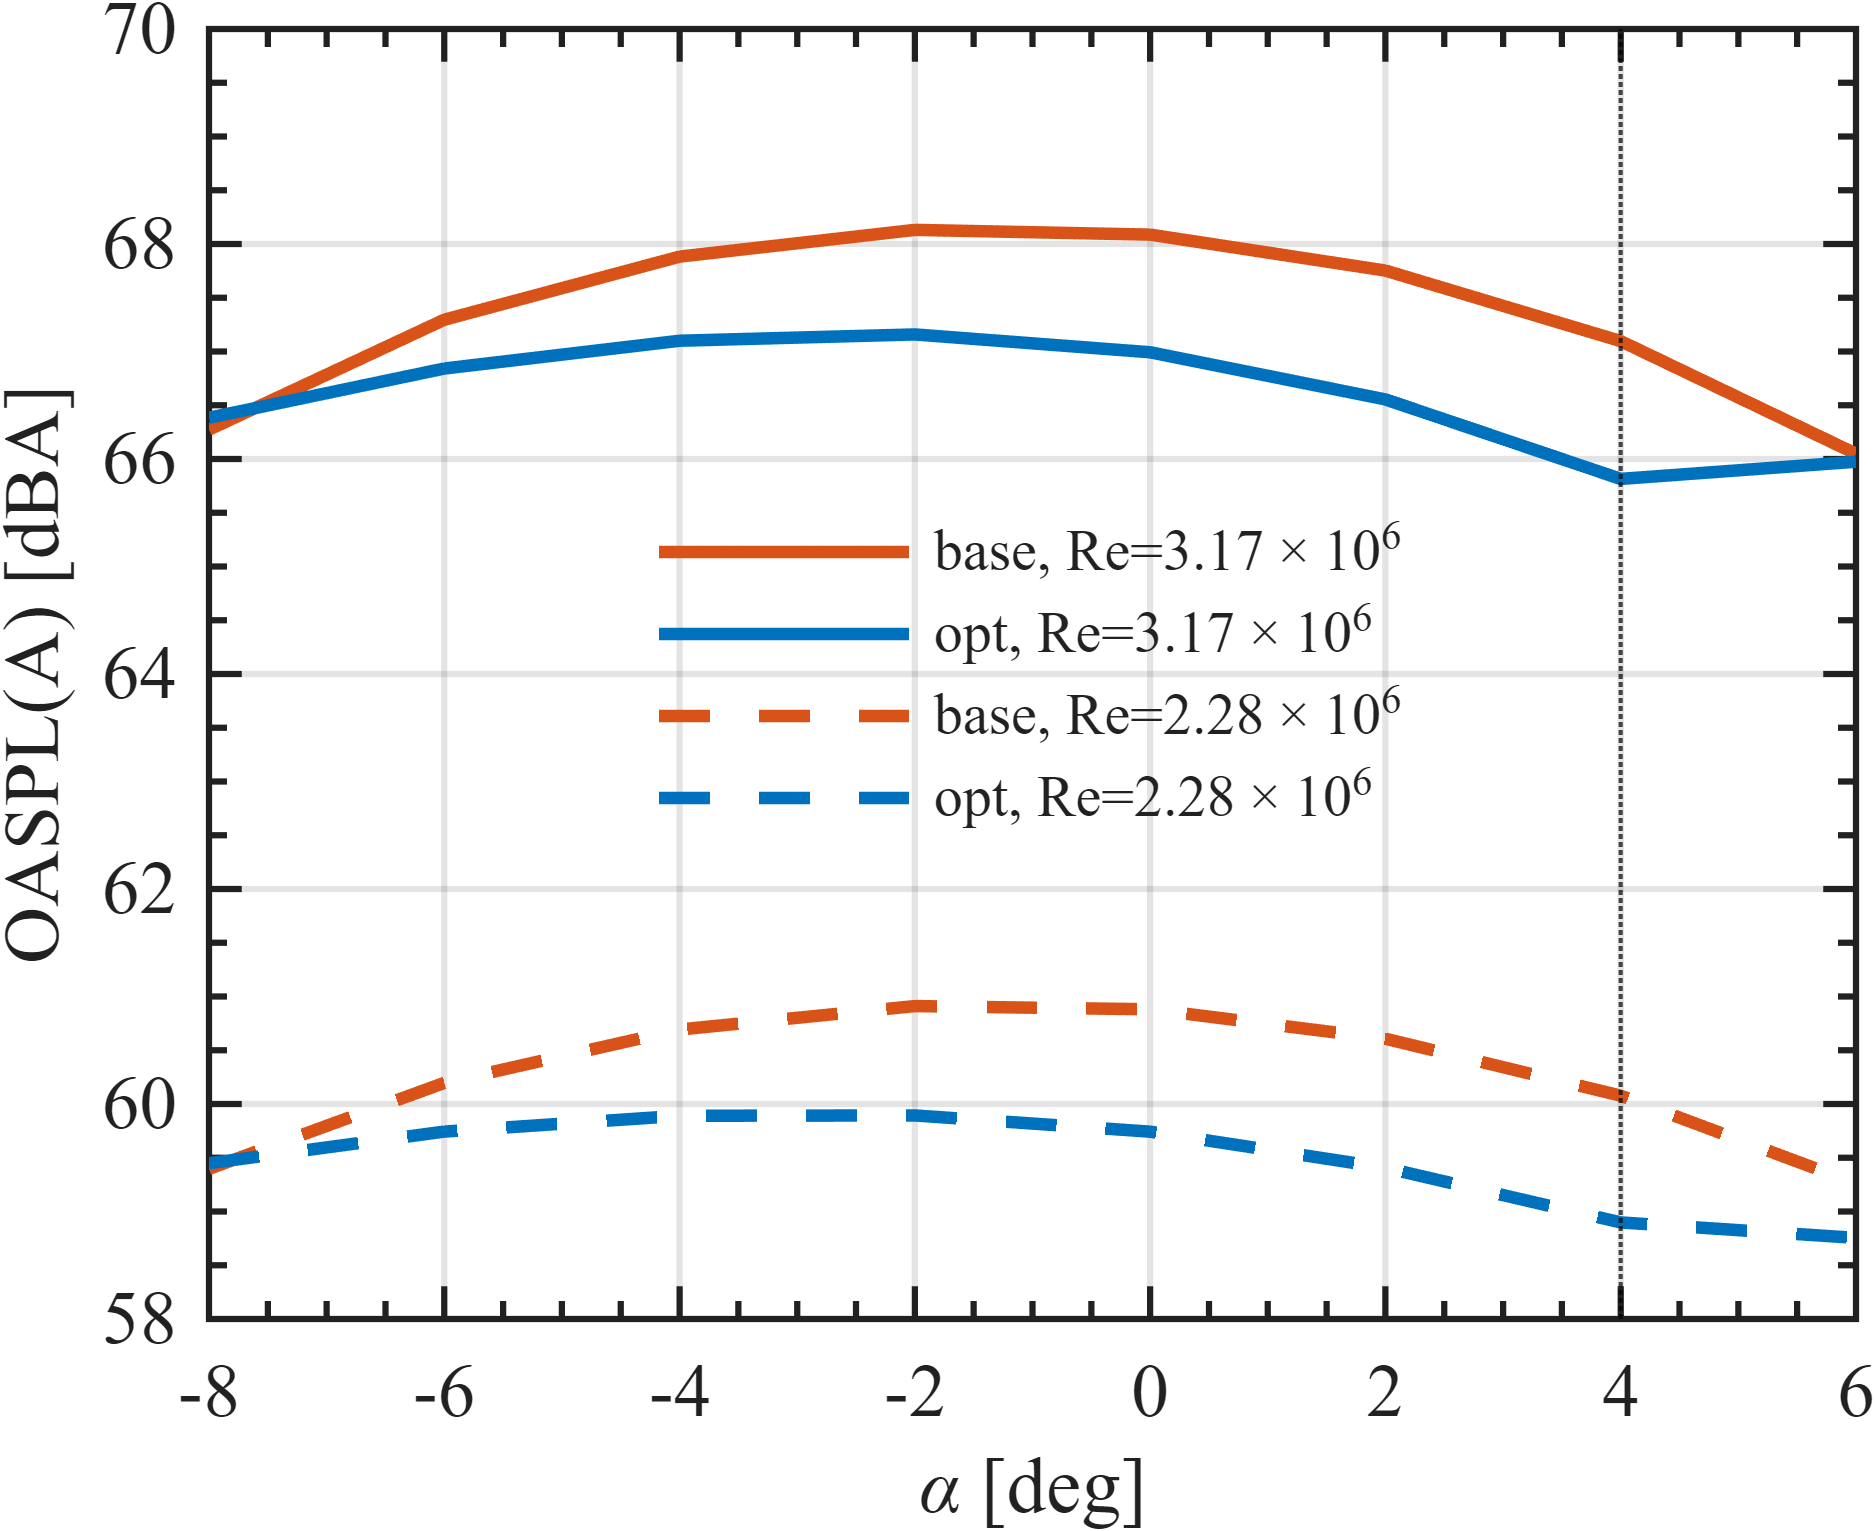
\includegraphics[width=\linewidth]{fig_offdesign_NACA63221.png}
\caption{}\end{subfigure}\hfill
\begin{subfigure}{0.48\linewidth}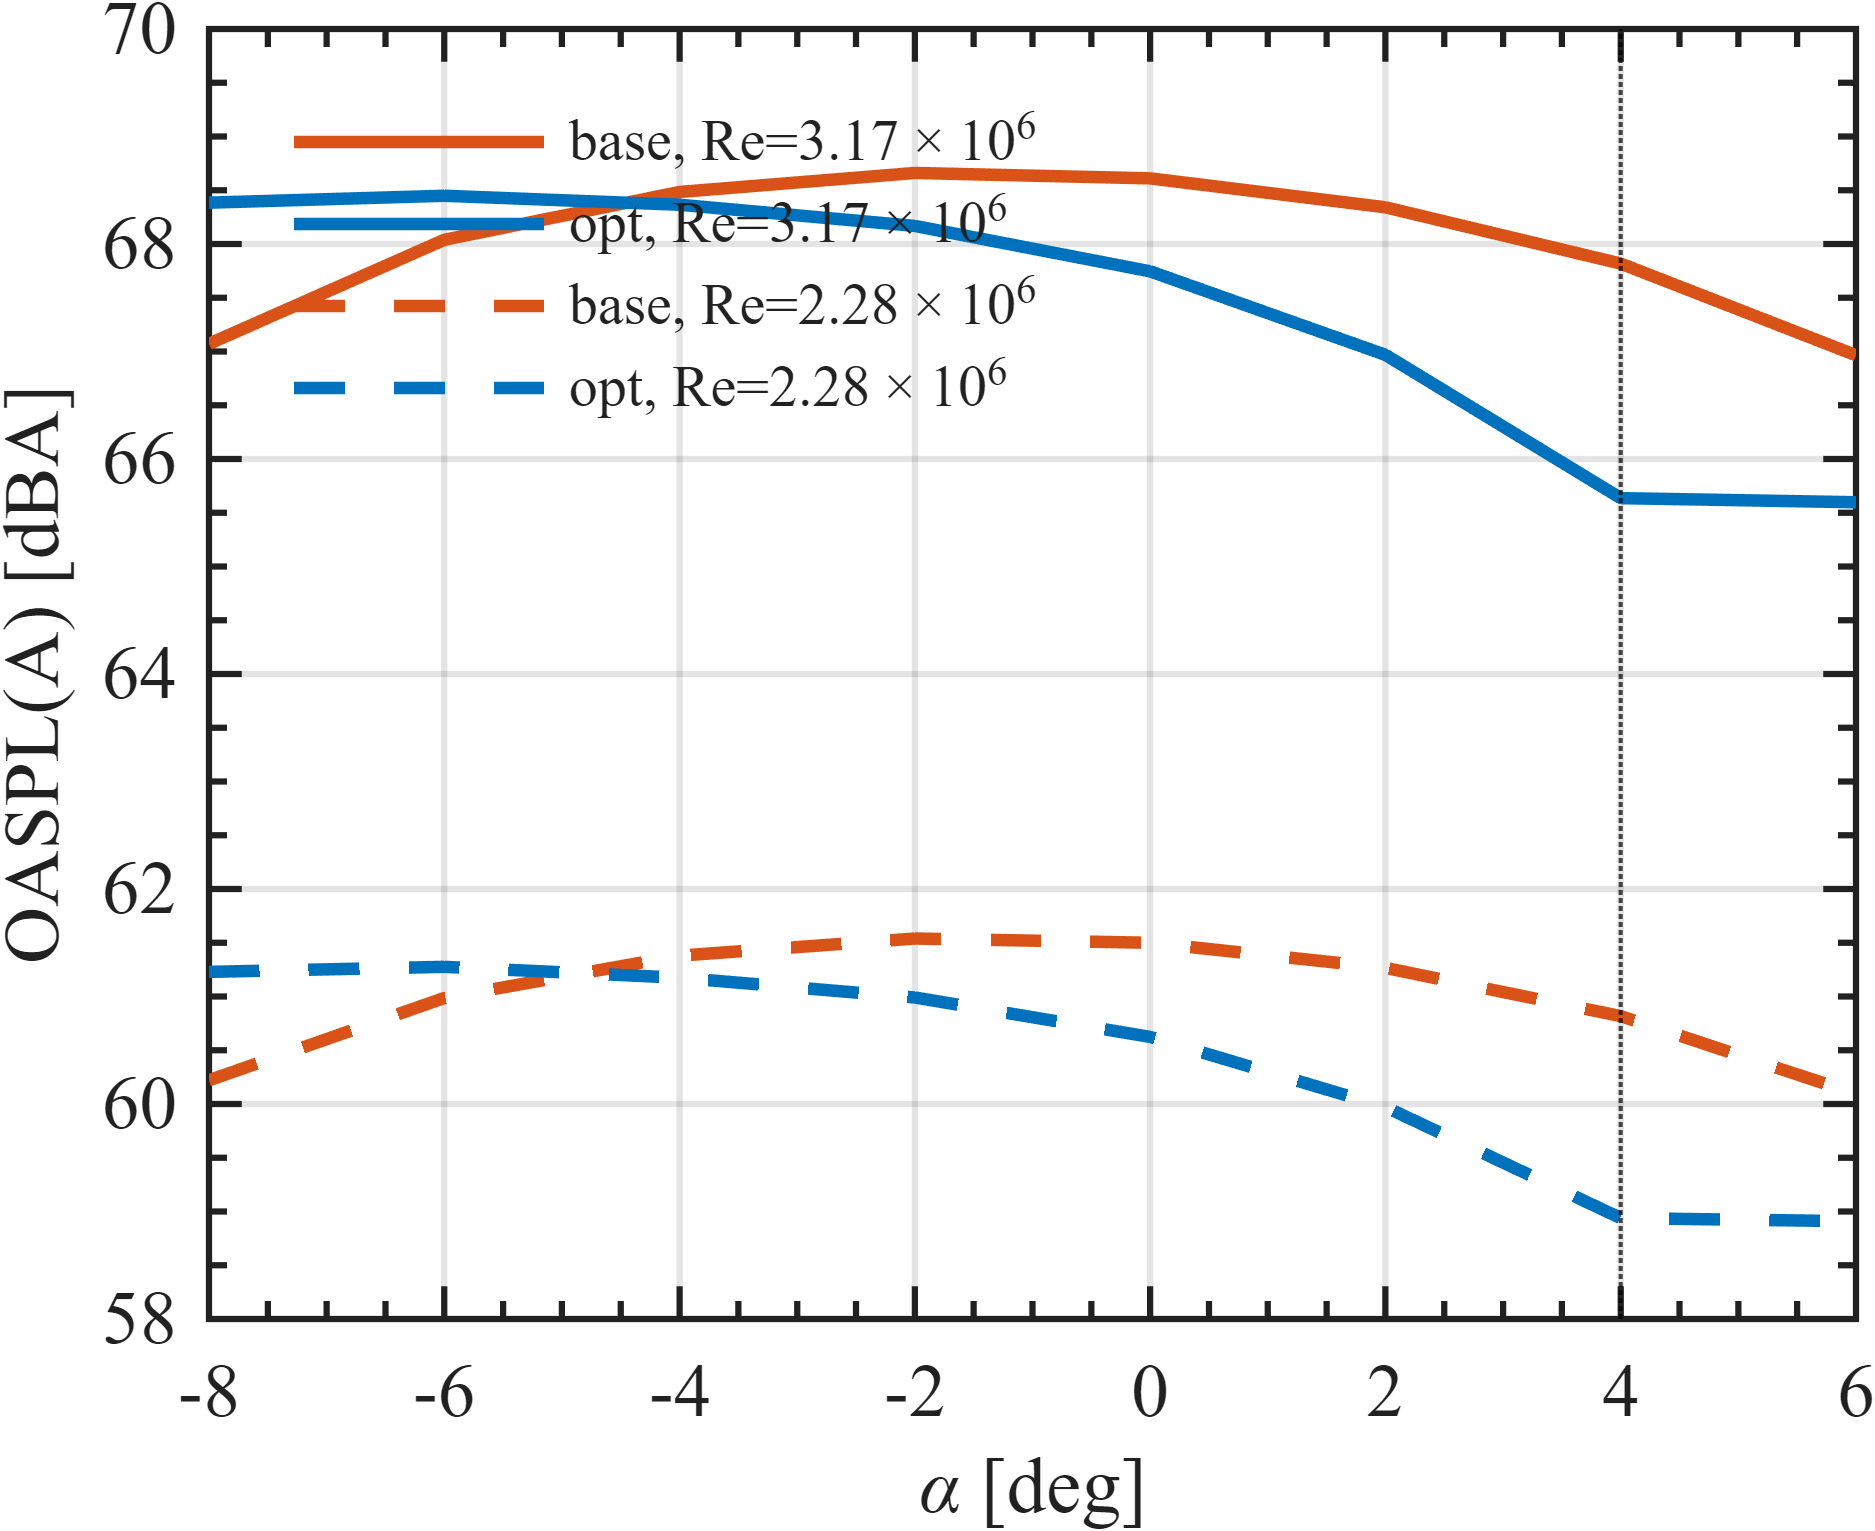
\includegraphics[width=\linewidth]{fig_offdesign_NACA63218.png}
\caption{}\end{subfigure}
\caption{Off-design behavior of the optima: OASPL(A) versus angle of attack
over $\alpha=-8$--$6^{\circ}$ at two Reynolds numbers for (a) NACA 63-221 and
(b) the robust NACA 63-218 optimum (orange: baseline, blue: optimum; solid:
$Re=3.17\times10^6$, dashed: $Re=2.28\times10^6$). Both optima stay quieter
over most of the range; the highly cambered 63-218 optimum loses and then
reverses its advantage at strongly negative incidence.}
\label{fig:offdesign}
\end{figure}

\subsection{Comparison with the literature}
Table~\ref{tab:lit} places the present results in the context of previous
aeroacoustic shape-optimization studies that use the same class of fast
noise-prediction models. The reduction obtained for the \SI{21}{\percent}
section is smaller than some reported values, which is expected for a thick
section with a strict attachment constraint and a bounded design box; as shown
above, the attainable figure depends on the allowed design freedom and on the
baseline section (the thinner 63-218, re-optimized with the robust multi-model
objective, yields \SIrange{1.9}{2.2}{dBA} confirmed across three wall-pressure
models). The added value of this work lies in the \emph{combination} of a
reconstruction-based parameterization screening, an optimizer benchmark, an
explicit wall-pressure model-uncertainty analysis and a robust multi-model
formulation that keeps the optimized boundary layer attached --- not in the
magnitude of the reduction alone, which depends strongly on the baseline airfoil
and the allowed design space.

\begin{table}[!htbp]\centering
\caption{Context of related TE-noise shape-optimization studies. Cases and
baselines differ, so the reductions are not directly comparable and are listed
only as orders of magnitude.}
\label{tab:lit}
\setlength{\tabcolsep}{4pt}
\begin{tabular}{@{}lllllll@{}}
\toprule
Study & Noise model & Case & Param. & Optimizer & Reduction & Evidence level \\
\midrule
\citet{Kou2023}            & Amiet+TNO & NACA0012 (airfoil) & CST  & PSO & \SI{1.11}{dBA} & numerical \\
\citet{Kou2023}            & Amiet+TNO & NACA0012 (airfoil) & VAE  & PSO & \SI{1.75}{dBA} & numerical \\
\citet{VolkmerCarolus2018} & Amiet+s.e.& airfoil            & spline & evol. & lift-pres. & numerical \\
\citet{Lee2013}            & BPM       & airfoil/blade      & --   & GA  & --           & experimental \\
\citet{RodriguesMarta2014} & BPM       & full blade         & --   & grad. & $\sim$\SI{10}{\percent} & numerical \\
\citet{WonLee2024}         & Amiet+WPS & rotor airfoil      & multiple & multi-obj. & -- & numerical \\
\textbf{Present work}      & Amiet+TNO & NACA 63-221 (airfoil) & CST & PS & \SI{1.28}{dBA} & WPS assessment \\
\textbf{Present work}      & Amiet+TNO & NACA 63-218 (airfoil) & CST & PS & \SIrange{1.9}{2.2}{dBA} & robust 3-model \\
\bottomrule
\end{tabular}
\end{table}

\subsection{Effect of the optimization on blade-radiated noise}\label{sec:blade}
%=======================================================================
% SECTION LEFT BLANK ON PURPOSE -- to be completed by a co-author.
% Intended content: how the sectional OASPL(A) reduction of the optimized
% tip section (NACA 63-218) propagates to the noise radiated by the FULL
% blade, via a blade-element + per-section Amiet spanwise integration.
% The blade far-field spectrum figure (baseline vs optimized) goes here once
% it is available and standardized to the paper palette:
%
% \begin{figure}[!htbp]\centering
% \includegraphics[width=0.7\linewidth]{fig_blade_noise.png}
% \caption{Far-field sound pressure level radiated by the baseline and
% optimized blade.}
% \label{fig:blade}
% \end{figure}
%=======================================================================
\TODO{To be written: effect of the sectional shape optimization on the noise
radiated by the complete blade (figure to be inserted).}

\FloatBarrier
%========================================================================
\section{Conclusions}\label{sec:concl}
%========================================================================
A framework for aeroacoustic airfoil shape optimization based on Amiet's theory,
the TNO--Blake wall-pressure model and XFOIL was used to minimize the A-weighted
OASPL of an airfoil under aerodynamic and geometric constraints. Unlike previous
studies, the framework was used to \emph{compare} design choices: CST gave the
lowest reconstruction error among the tested parameterizations and was therefore
selected for the optimization, a
sensitivity analysis showed that the aft CST coefficients dominate the variation
of the objective, and five optimization algorithms were benchmarked on the same
problem. A ten-seed repetition of the stochastic solvers showed their
distributions to overlap within their seed scatter ($\sigma\le\SI{0.18}{dBA}$),
with no clear winner --- the single-run advantage of the genetic algorithm did
not survive repetition, particle swarm and surrogate optimization being
marginally better on average;
the gradient-based SQP did not stagnate on this constrained problem
(\SI{0.85}{dBA}); and pattern search, although the least effective at that
small budget (\SI{0.55}{dBA}), was adopted as the dedicated single-objective
optimizer and, at a larger budget, mesh-converged to \SI{65.82}{dBA} --- below
every solver's single 150-evaluation run (Table~\ref{tab:algo}), though a
single favorable particle-swarm seed reached a marginally lower value
(\SI{65.65}{dBA}, Table~\ref{tab:seeds}). For the present case, the attainable reduction showed a
strong dependence on the evaluation budget, while the differences among
solvers at the nominal 150-evaluation budget were smaller; the dedicated
optimum is therefore reported as the headline result. Within the TNO--Blake
prediction framework, the tested
$\pm50\%$ CST design box and the single prescribed operating point, the
optimized NACA 63-221 reduces the \emph{predicted} OASPL(A) by
\SI{1.28}{dBA} (about \SI{26}{\percent} of the A-weighted mean-square
acoustic pressure) while approximately preserving the maximum thickness
($t_{\max}/c$ $0.210\!\to\!0.205$) and slightly improving its lift-to-drag
ratio (from $54.2$ to $54.8$); the pressure-gradient-sensitive Kamruzzaman
model does not confirm this trend (Section~\ref{sec:sens}), so the figure is
conditional on the wall-pressure model. For this thick section the \emph{pressure} side is the
dominant far-field source, yet the optimization acts on both surfaces, with the
quieter suction side carrying the larger share of the energy reduction.
Progressively widening the design box
($\pm30\%\!\to\!\pm50\%\!\to\!\pm70\%$) increases the reduction ($1.02$, $1.28$
and \SI{1.74}{dBA}), wider boxes admitting geometries progressively further
from the 63-221 family; the $\pm50\%$ box is thus a design choice balancing
noise reduction against geometric fidelity, and within it the
efficiency-unconstrained multi-objective front bottoms out at the level of the
constrained optimum.

Applied to the thinner NACA 63-218 section of the same family, the framework
was recast with a \emph{robust multi-model} objective (minimizing the worst
case among the TNO, Goody and Kamruzzaman wall-pressure models) over an
expanded design box. The resulting \SI{18}{\percent} optimum reduces the
predicted noise in all three wall-pressure models simultaneously
($2.18$, $2.04$ and \SI{1.91}{dBA}) while improving the lift-to-drag ratio
(from $60.1$ to $63.2$), through the same constant-thickness forward-camber
mechanism as the 63-221 (maximum thickness essentially preserved, maximum
camber roughly sextupled and shifted forward). It therefore \emph{dominates}
the baseline while preserving an approximately \SI{18}{\percent} maximum
thickness and, unlike single-model optimization, its predicted benefit is
consistent across the three wall-pressure models considered --- the robust
formulation directly addresses the model-form uncertainty that a post-hoc
model comparison had exposed for single-model optima; re-optimizing with a
relative worst-case objective (each model referred to its own baseline)
confirmed this result and slightly improved the balance of the reductions
across the three models. The main
caveat is a reduced negative-incidence
margin: the added camber makes the acoustic advantage diminish toward low
incidence and reverse at negative angles, which must be verified against gust
requirements before use on a blade.

A central element of the formulation is the attachment constraint. Because the
TNO wall-pressure model assumes an attached turbulent boundary layer, a
suction-side constraint (shape factor $H\le2.7$ and skin friction
$C_f\ge1.5\times10^{-4}$ at $x/c=0.99$) was imposed; without it, the optimizer
lowers the predicted wall pressure by driving the suction side toward
separation, where the model is invalid and the predicted reduction is spurious.
With the constraint, the reported optimum keeps the suction-side boundary layer
attached (the shape factor rises from $2.26$ to $2.62$), so the noise
reduction rests on physically admissible boundary layers. Because the
optimum sits exactly on the $C_{f,\min}$ floor, part of the reported figure
may depend on the chosen thresholds; a sensitivity study over $C_{f,\min}$
and $H_{\lim}$, and enforcement of the constraint on both surfaces over the
whole chord, are identified as necessary refinements. The fast-prediction
optimization studies reviewed here do not consistently report an explicit
attachment constraint.

Several limitations remain. The noise is predicted with a fast semi-empirical
chain (XFOIL + TNO--Blake + Amiet) whose TNO model under-predicts the
high-frequency wall pressure; because this deviation is frequency-dependent, the
A-weighted reduction can differ from a higher-fidelity prediction. This
sensitivity was quantified in Section~\ref{sec:sens}: for the single-model
optima the Goody model confirms the reduction while the Kamruzzaman model does
not; the robust multi-model optimization of the 63-218
(Section~\ref{sec:63218}) restores agreement across the three
wall-pressure models, so its figure is no longer conditional on a single
model, although higher-fidelity confirmation is still needed. This need is
underscored by \citet{Barry2026}, who found that a fast TBL--TE + Amiet model,
while reproducing a baseline reasonably, can deviate by up to \SI{9}{dB} from a
lattice-Boltzmann evaluation for the \emph{optimized} geometries --- so the
optima, not only the baseline, should be validated at higher fidelity.
Wall-pressure models that
explicitly account for the adverse pressure
gradient \citep{Rozenberg2012,LeeShum2019} or for non-equilibrium boundary
layers \citep{Pargal2024} could improve the absolute prediction. The
optimization is carried out at a single operating condition; the post-hoc
sweep of Section~\ref{sec:sens} shows that the gains persist over
$\alpha=2$--$6^{\circ}$ (63-218, with a reduced negative-incidence margin) and
$2$--$5^{\circ}$ (63-221) and at a lower
Reynolds number, but roughness and inflow turbulence remain untested,
independent Mach-number effects were not isolated (Mach co-varied with
Reynolds through the inflow velocity), and the objective is still
single-point. The thickness constraint caps the maximum thickness but
enforces only a loose minimum-thickness floor (a geometric, not structural,
bound): the 63-221 and the robust 63-218 optima stay close to their
baseline maximum thickness (the 63-221 within \SI{2.4}{\percent} of the cap,
the robust 63-218 at \SI{18}{\percent}), but several Pareto designs are markedly
thinner than their baselines and would have to be checked against the structural
requirements of the corresponding blade station. Aerodynamic moment, leading-edge radius and
manufacturability are also
not constrained; the pitching-moment magnitude decreases for the
single-objective optima but grows for some Pareto designs, and the robust
63-218 optimum has a reduced negative-incidence margin owing to its added
camber. The optimized
airfoils are therefore
noise-reduction demonstrations rather than design-ready wind-turbine blade
sections. Future work includes
multiple-angle-of-attack and multi-point objectives, a tighter
structural minimum-thickness constraint, and machine-learning parameterizations
such as variational autoencoders.

%========================================================================
\section*{CRediT authorship contribution statement}
\textbf{Jose Antonio Parada Marin:} Conceptualization, Methodology, Software,
Investigation, Writing -- original draft. \textbf{Laura Botero-Bol\'ivar:}
Conceptualization, Methodology, Supervision, Writing -- review \& editing.
\textbf{Octavio Andr\'es Gonz\'alez-Estrada:} Supervision, Resources,
Writing -- review \& editing.

\section*{Declaration of competing interest}
The authors declare no competing interests.

\section*{ORCID}
Jose Antonio Parada Marin: 0000-0002-7930-2479.
Laura Botero-Bol\'ivar: 0000-0002-9824-1173.
Octavio Andr\'es Gonz\'alez-Estrada: 0000-0002-2778-3389.

\section*{Funding}
This research received no external funding.

\section*{Data and code availability}
The baseline and optimized airfoil coordinates, the CST coefficients of all
reported optima, the optimization histories and the driver scripts supporting
this study are available from the corresponding author upon reasonable
request.

\FloatBarrier

\bibliographystyle{elsarticle-num-names}
\bibliography{refs}

\end{document}
